% !TEX encoding = UTF-8
% !TEX TS-program = pdflatex
% !TEX root = ../thesis.tex

%************************************************
\chapter{Computational Details}\label{chap:5:computational_details}
%************************************************

Our final goal is clear now: We want to investigate the effect of finite top- and bottom-quark masses on the Higgs production cross section, both on the inclusive and the differential cross section level. In particular, we want to study the impact of the mass renormalization scheme on the cross section to eliminate one of the main remaining uncertainties of the cross section. Furthermore, in addition to the commonly used 5\acs{FS}, we want to explore the impact of alternative \acs{FS}s to assess the validity of the treatment of light quark masses in the 5\acs{FS}.

In this chapter, we will describe the necessary methods for computing the Higgs production cross section with full top- and bottom-quark mass dependence at \acs{NNLO}.

\section{Computing the Amplitudes}
The base ingredients of the calculation are the scattering amplitudes. In addition to the \acs{LO} amplitude for $gg \rightarrow H$ presented in section~\ref{sec:4:LO_xSec} and the \acs{NLO} amplitudes computed in Ref.~\cite{Graudenz:1992pv}, we require amplitudes for the following partonic processes
\begin{itemize}
  \item Real-Real Corrections (One-loop):
  \begin{enumerate}
    \item $gg \rightarrow H gg$
    \item $gg \rightarrow H q \bar{q}$
    \item $q\bar{q} \rightarrow H q^\prime \bar{q}^\prime$
    \item + processes related by crossing symmetry
  \end{enumerate}
  \item Real-Virtual Amplitudes (Two-loop):
  \begin{enumerate}
    \item $gg \rightarrow Hg$
    \item $q \bar{q} \rightarrow H g$
    \item + processes related by crossing symmetry
  \end{enumerate}
  \item Virtual-Virtual Amplitudes (Three-loop):
  \begin{enumerate}
    \item $g g \rightarrow H$.
  \end{enumerate}
\end{itemize}
In the following, we discuss the computation of each element one-by-one.

In this section, we are exclusively working in the 5\acs{FS}. The necessary modifications for adapting the amplitudes to the 4\acs{FS} will be presented in section~\ref{sec:5:4FS}. When working in the 5\acs{FS}, the bottom-quark mass is generally zero. Since this would imply that the total top-bottom interference contribution is vanishing, one then sets the mass to its actual value inside all closed quark loops that couple to the Higgs. Therefore in Feynman diagrams like those depicted in Fig.~\ref{fig:5:real_virtual2}, the bottom quark is treated as massive, but if the top- and bottom-quark are exchanged, the bottom quark mass is set to zero. With a massification prescription like this, it is essential to verify that gauge invariance and \acs{IR} safety are not lost in the process.

The proof that it is not proceeds by the replica technique. Consider the \acs{SM} but only with the following quark content: $n_b$ identical copies of the bottom quark, $n_{b^\prime}$ massless quarks $b^\prime$ serving as our massless bottom quark, and the top-quark. Without the inclusion of electroweak effects this theory is equivalent to \acs{QCD} with the addition of a Yukawa interaction to the Higgs; ergo this theory is gauge invariant and free of \acs{IR}-divergences. Furthermore, gauge invariance and \acs{IR}-safety also hold for each individual Yukawa coupling contribution ($Y_t$ or $Y_b$) and each power of $n_b$ and $n_{b^\prime}$, as these are arbitrary parameters from the point of \acs{QCD}. This means that the parts of the amplitude which are proportional to $Y_t n_b$ are separately gauge invariant, and so are the parts which are proportional to $Y_b n_b n_{b^\prime}$, and so on. Examples of Feynman diagrams contributing to a selection of $Y_t$, $Y_b$, $n_b$ and $n_{b^\prime}$ power-combinations are depicted in Fig.~\ref{fig:5:replica}.
\begin{figure}[h]
\centering
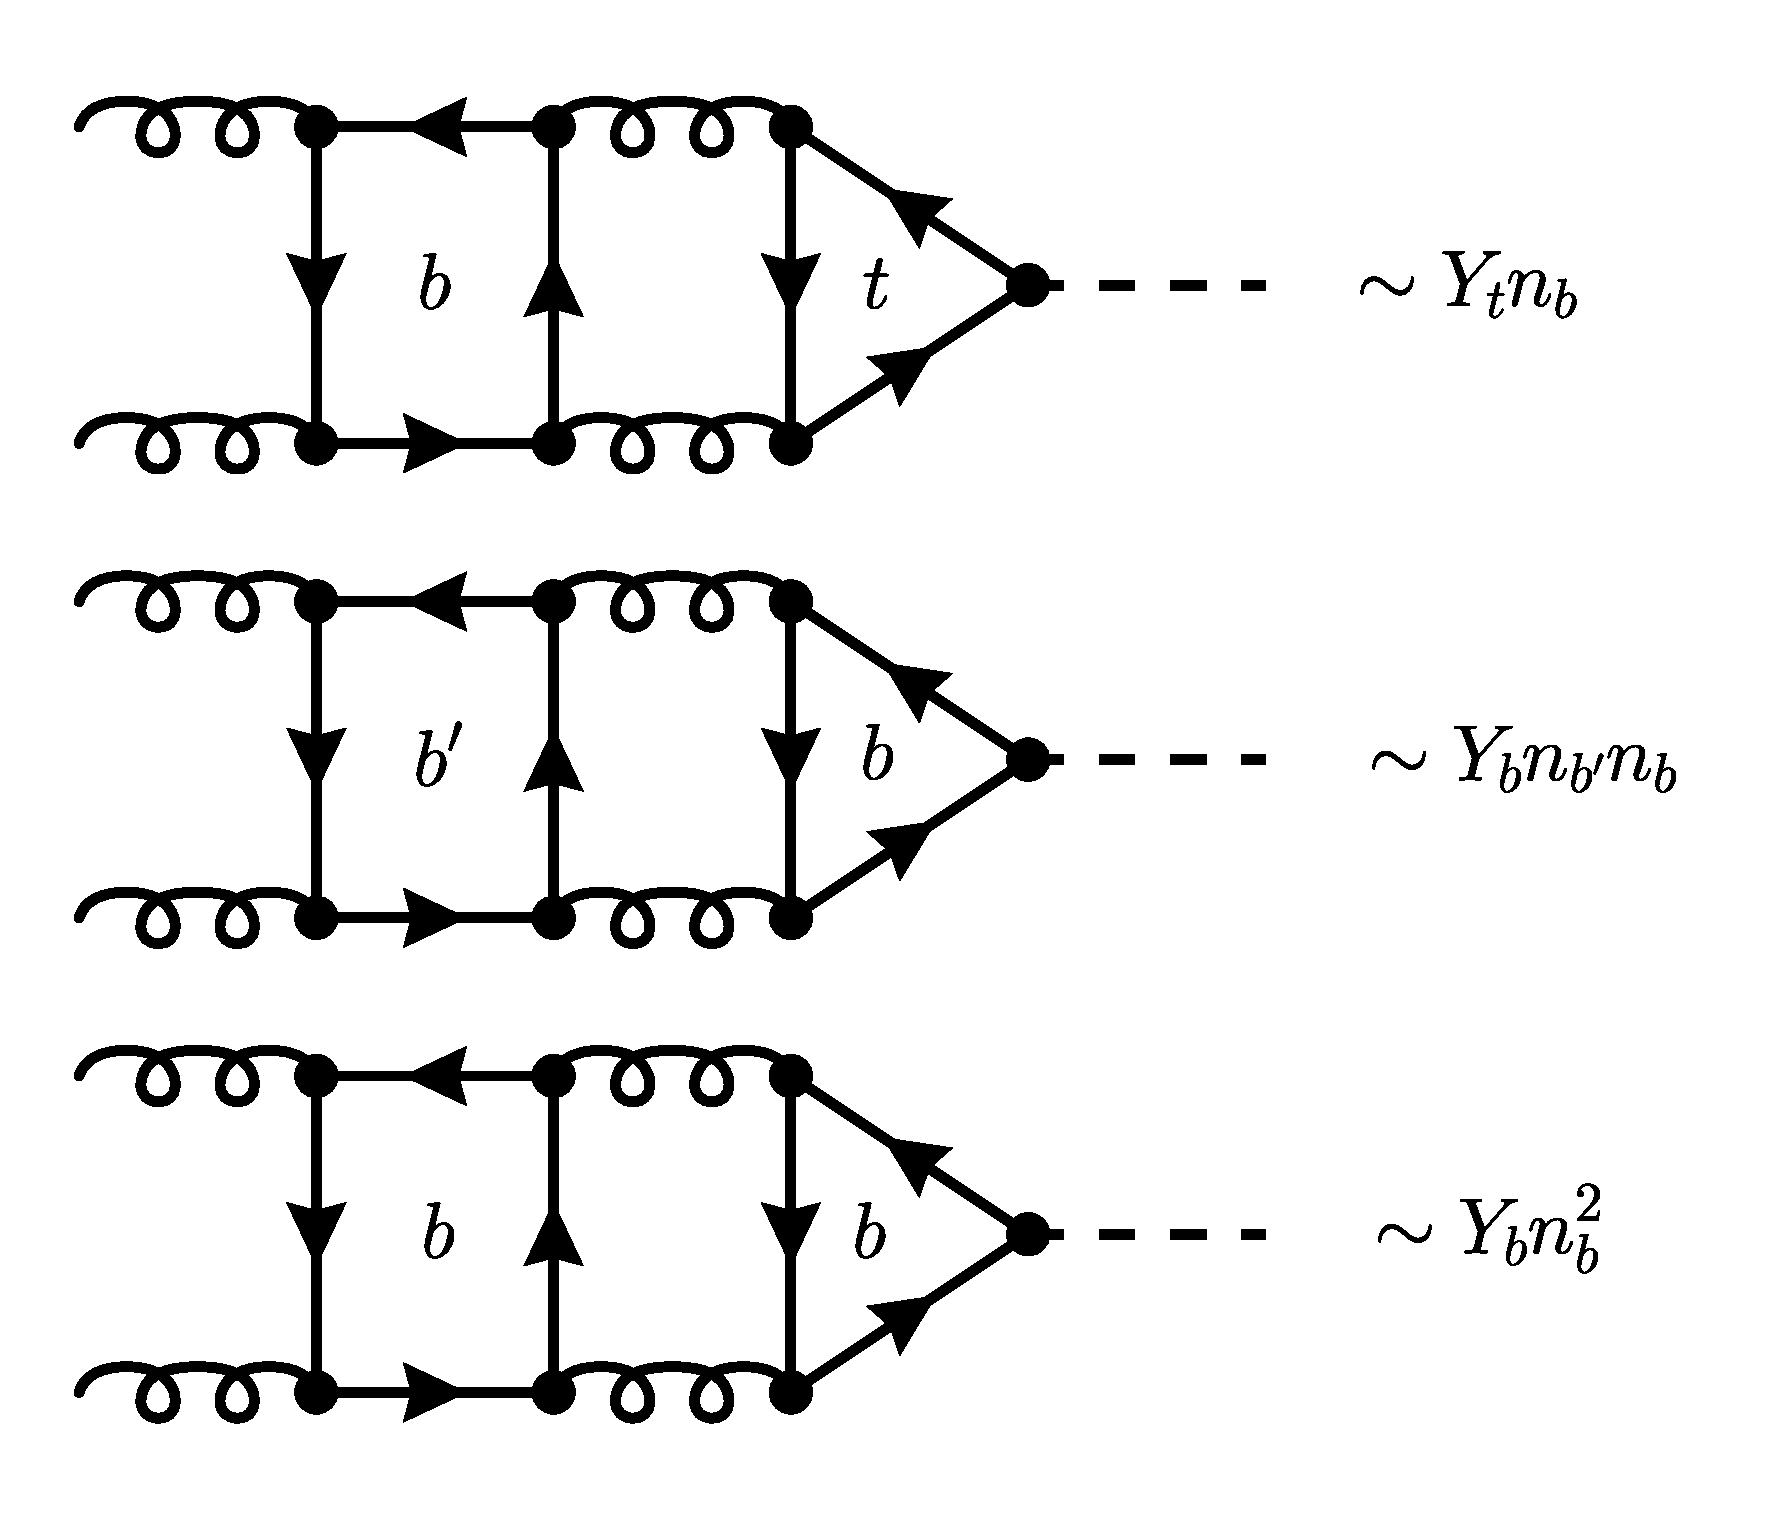
\includegraphics[scale=0.21]{Images/NNLO_Feynman_diagrams/replica.pdf}
\caption{Example Feynman diagrams and their scaling with the Yukawa coupling, $n_b$, and $n_{b^\prime}$.}
\label{fig:5:replica}
\end{figure}
Likewise, after squaring, the contribution $Y_t Y_b n_{b^\prime} n_{b}$ is going to be separately \acs{IR} finite. We have thus shown, that contributions with a massive bottom-quark loop which does \textbf{not} couple to the Higgs does not mix gauge dependent terms or \acs{IR} divergences with the selected contribution from our massification procedure.

\subsection{The Real-Real Corrections}
The real-real corrections only contain a single loop, with either a top or a bottom quark running in the loop. Examples of different Feynman diagrams for various partonic channels are depicted in Fig.~\ref{fig:5:real_real}.
\begin{figure}[h]
  \centering
  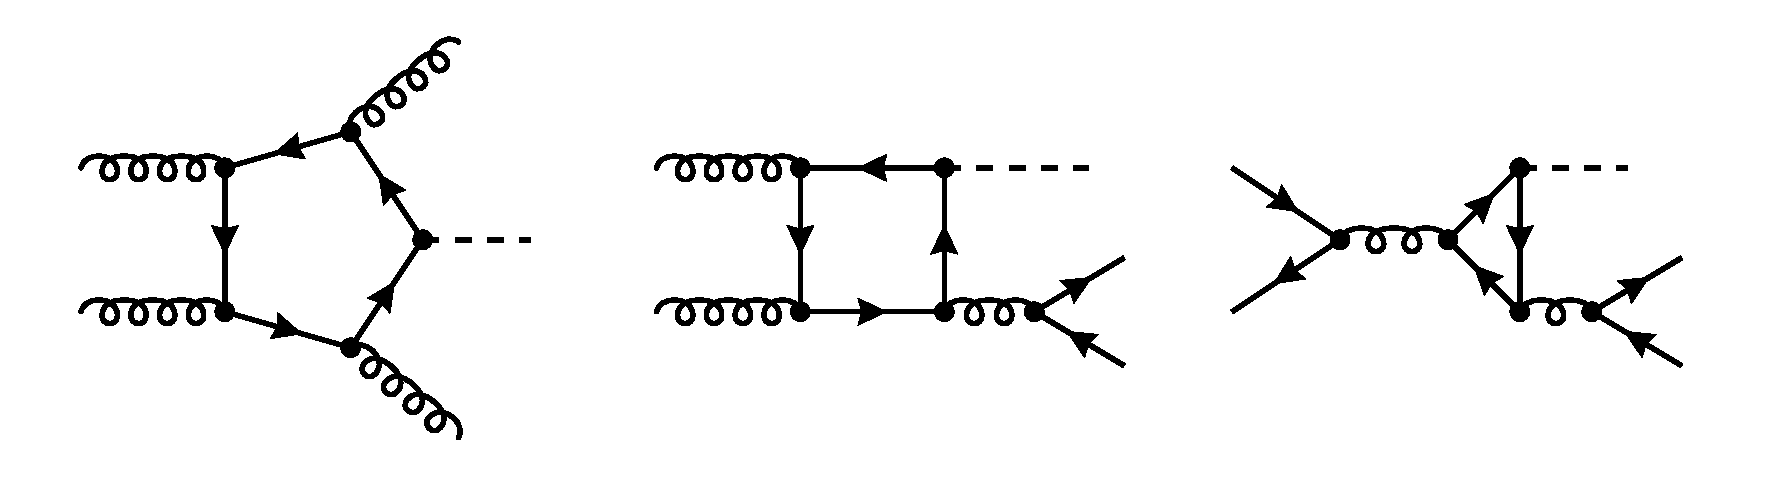
\includegraphics[width=\figurewidth]{Images/NNLO_Feynman_diagrams/RealReal.pdf}
  \caption{Example Feynman diagrams for one-loop real-real corrections in various partonic channels.}
  \label{fig:5:real_real}
\end{figure}

As one-loop amplitudes, they can be computed numerically with publically available libraries like \texttt{Recola}~\cite{Actis:2016mpe}. However, the real-real corrections often represent the bottleneck of the computation of the phase-space integrals, which makes an efficient evaluation of the amplitudes desirable. We therefore instead use the analytic form of the amplitude computed in Ref.~\cite{Budge:2020oyl}. We use the implementation of the amplitudes provided by \texttt{MCFM}~\cite{Campbell:2019dru, Campbell:1999ah, Campbell:2011bn}, which in turn uses \texttt{QCDLoop}~\cite{Ellis:2007qk, Carrazza:2016gav} for the evaluation of one-loop integrals.

We found that with the analytic expressions, the evaluation time of the amplitudes is sped up by a factor of 20 compared to the numerical evaluation in \texttt{Recola}.

\subsection{The Real-Virtual Corrections} \label{subsec:5:the_real-virtual_corrections}
For the real-virtual corrections we, for the first time encounter Feynman diagrams with two different mass scales running in the loop. Fig.~\ref{fig:5:real_virtual2} shows all (up to inversion of the fermion flow inside the triangle loops) Feynman diagrams with two internal quark loops.
\begin{figure}[h]
  \centering
  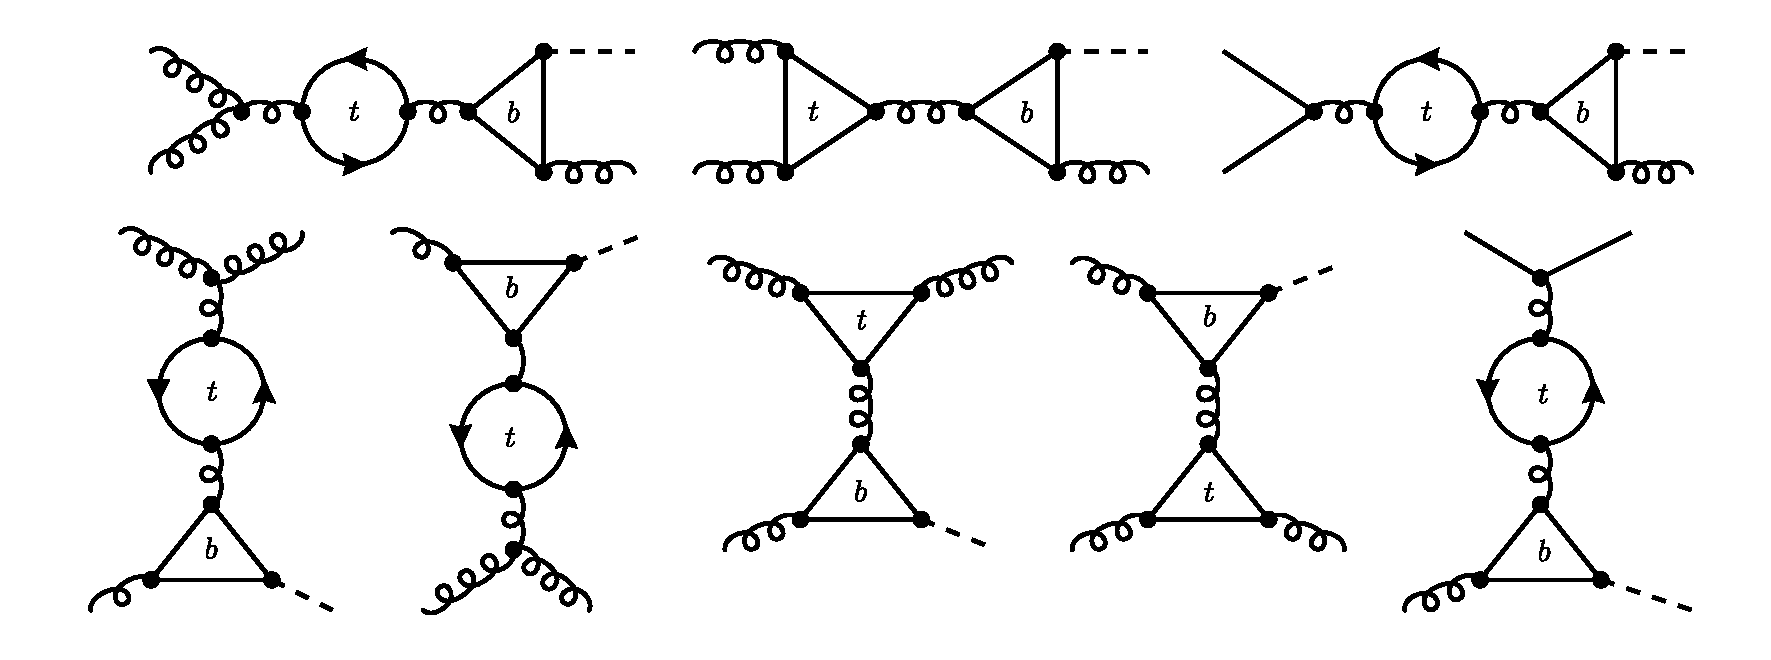
\includegraphics[scale=0.5]{Images/NNLO_Feynman_diagrams/RealVirtual2.pdf}
  \caption{Feynman diagrams for the two-loop real-virtual corrections with two massive quarks. Amplitudes for the $qg \rightarrow Hq$ channel can be obtained via crossing from the $q \bar{q} \rightarrow H g$ amplitudes.Triangle loops with reversed fermion flow are not explicitly shown. The external gluons must be accounted for with all permutations which render a different Feynman diagrams. In the 5\acs{FS}, the bottom-quark is always coupling to the Higgs.}
  \label{fig:5:real_virtual2}
\end{figure}
We observe, that all two-loop integrals actually factorize into two separate one-loop integrals making them quite straight-forward to solve.

The contributions to the scattering amplitude containing only a single massive quark involve genuine two-loop integrals. Fig.~\ref{fig:5:real_virtual1} shows a selection of contributing Feynman diagrams.
\begin{figure}[h]
  \centering
  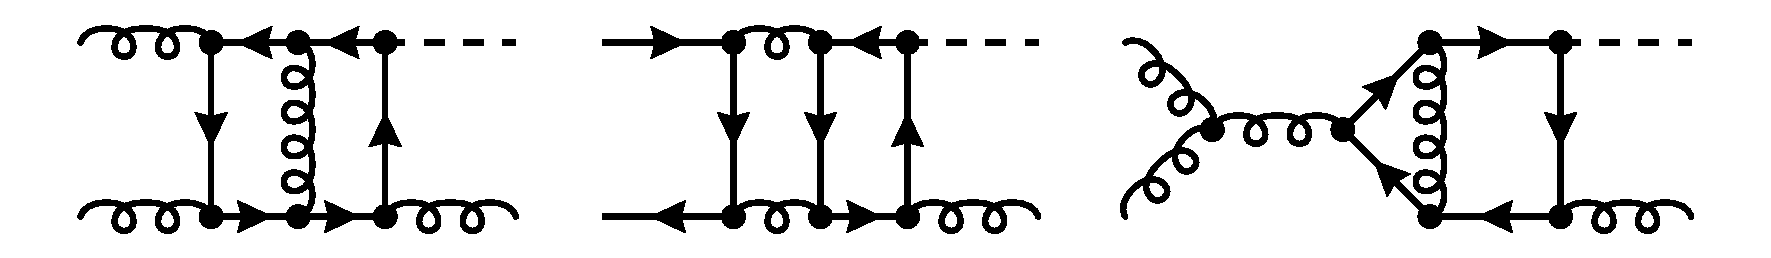
\includegraphics[width=\figurewidth]{Images/NNLO_Feynman_diagrams/RealVirtual1.pdf}
  \caption{Example Feynman diagrams for the two-loop real-virtual corrections with a single massive quark in various partonic channels.}
  \label{fig:5:real_virtual1}
\end{figure}
Two loop integrals, especially non-planar ones, with three mass scales are very challenging to compute analytically, even with state-of-the-art methods, and as of today the analytic computation of these amplitudes are still unknown, however approximations for a nearly massless bottom quark have been calculated relatively recently~\cite{Melnikov:2016qoc, Melnikov:2017pgf}. We therefore decided to instead evaluate the appearing two-loop integrals numerically at fixed phase-space points and interpolate between them during the phase-space integration.

In any case, for both the one-mass and two-masses contribution we first have to reduce the amplitude to form factors. To make possible symmetries more apparent, we cross the radiated parton to the initial state, \ie\ we consider the amplitudes
\begin{equation}
g(p_1) + g_(p_2) + g(p_3) \longrightarrow H(p_4), \qquad \bar{q}(p_1) + q(p_2) + g(p_3) \longrightarrow H(p_4).
\end{equation}

\textbf{Projection to Form Factors}\\
We can factor out the external polarization vectors, spinors and color factors to rewrite the amplitudes in terms of their amputated counterpart
\begin{equation}
\mathcal{M}_{ggg \rightarrow H} = \mathcal{M}_{\mu \nu \rho} \epsilon_1^\mu \epsilon_2^\nu \epsilon_3^\rho f^{c_1 c_2 c_3}, \qquad \mathcal{M}_{\bar{q} q g \rightarrow H} = \bar{v}(p_1) \mathcal{M}_{\rho} u(p_2) \epsilon_3^\rho T^{c_3}_{c_1 c_2}.
\end{equation}
After squaring the amplitude and summing over the color of the external partons, we get the color factors
\begin{equation}
f^{c_1 c_2 c_3} f^{c_1 c_2 c_3} = C_A N_A = 24, \qquad T^{c_3}_{c_1 c_2} T^{c_{3}}_{c_2 c_1} = C_F N_c = 4.
\end{equation}
It is convenient, to choose polarization vectors which are cyclically transverse to the external momenta, \ie\
\begin{equation}
\epsilon_1 = \epsilon (p_1; p_2), \quad \epsilon_2 = \epsilon (p_2; p_3), \quad \epsilon_3 = \epsilon (p_3; p_1),
\end{equation}
where the second argument indicates the gauge vector. We can then propose the form factor decomposition of the amplitudes
\begin{equation}
\begin{split}
\mathcal{M}^{\mu \nu \rho} &= g^{\mu \nu} p_2^\rho F_1 + g^{\mu \rho} p_1^\nu F_2 + g^{\nu \rho} p_3^\mu F_3 + p_3^\mu p_1^\nu p_2^\rho F_4, \\
\bar{v}(p_1) \mathcal{M}^{\rho} u(p_2) &= \bar{v}(p_1)\left[ \slashed{p}_3 p_1^\rho - (p_1 \cdot p_3) \gamma^\rho \right] u(p_2) G_1 + \bar{v}(p_1) \left[ \slashed{p}_3 p_2^\rho - (p_2 \cdot p_3) \gamma^\rho \right] u(p_2) G_2.
\end{split}
\end{equation}
We used the Ward identity, to restrict the tensor coefficients in $\mathcal{M}^\rho$. $\mathcal{M}^{\mu \nu \rho}$ also satisfies Ward identity.

The tensor coefficients span a vector space with respect to the scalar product
\begin{equation}
\braket{a_{\mu_1, \cdots \mu_{n_g}}| b^{\mu_1, \cdots \mu_{n_g}}} \equiv \sum_{\text{pol.}} a^*_{\mu_1 \ldots \mu_{n_g}} \left[\prod_i^{n_g} \epsilon_i^{*\mu_i} \epsilon_i^{\nu_i}  \right]  b_{\nu_1 \ldots \nu_{n_g}}
\label{eq:5:scala_product}
\end{equation}
where $n_g$ is the number of external gluons, \ie $n_g = 3$ for $ggg \rightarrow H$ and $n_g = 1$ for $\bar{q} q g \rightarrow H$ and the summation is performed over the polarizations of all external particles. The tensor coefficients hence form a---not necessary orthonormal---basis.

Any vector can be written as a linear sum over basis vectors
\begin{equation}
\ket{v} = \sum_i v_i \ket{e_i}.
\end{equation}
Then the projector to the $j$-th basis vector can be found via
\begin{equation}
\bra{e_j}P \equiv P_j = \sum_k G^{-1}_{jk} \ket{e_k},
\end{equation}
where $G$ is the Gram-matrix
\begin{equation}
G_{ij} = \braket{e_i | e_j}.
\end{equation}

With this little interlude from linear algebra it is then easy to verify that the projectors for the $F_1,\ldots , F_4$ form factors are given by
\begin{equation}
\begin{split}
P_1^{\mu \nu \rho} &= \frac{1}{d - 3} \left( g^{\mu \nu} p_2^\rho \frac{t}{su} - p_3^\mu p_1^\nu p_2^\rho \frac{1}{su} \right), \\
P_2^{\mu \nu \rho} &= \frac{1}{d - 3} \left( g^{\mu \rho} p_1^\nu \frac{u}{s t} - p_3^\mu p_1^\nu p_2^\rho \frac{1}{st} \right), \\
P_3^{\mu \nu \rho} &= \frac{1}{d - 3} \left( g^{\nu \rho} p_3^\mu \frac{s}{t u} - p_3^\mu p_1^\nu p_2^\rho \frac{1}{t u} \right), \\
P_4^{\mu \nu \rho} &= \frac{1}{d - 3} \left( - g^{\mu \nu} p_2^\rho \frac{1}{s u} - g^{\mu \rho} p_1^\nu \frac{1}{s t} - g^{\nu \rho} p_3^\mu \frac{1}{t u} + p_3^\mu p_1^\nu p_2^\rho \frac{d}{s t u} \right).
\end{split}
\end{equation}
To be even more explicit: the form factors are given by
\begin{equation}
\begin{split}
&F_i = \braket{e_i| P_{\mu \nu \rho} | \mathcal{M}^{\mu \nu \rho}} = P_i^{\mu_1 \nu_1 \rho_1} \left(-g_{\mu_1 \mu_2} + \frac{p_{1\, \mu_1} p_{2\, \mu_2} + p_{2\, \mu_1} p_{1\, \mu_2}}{p_1 \cdot p_2} \right) \\
& \qquad \times \left(-g_{\nu_1 \nu_2} + \frac{p_{2\, \nu_1} p_{3\, \nu_2} + p_{3\, \nu_1} p_{2\, \nu_2}}{p_2 \cdot p_3} \right) \left(-g_{\rho_1 \rho_2} + \frac{p_{3\, \rho_1} p_{1\, \rho_2} + p_{1\, \rho_1} p_{3\, \rho_2}}{p_3 \cdot p_1} \right) \mathcal{M}^{\mu_2 \nu_2 \rho_2}.
\end{split}
\end{equation}
Here we used the standard identity
\begin{equation}
\sum_{\lambda} \epsilon^{*}_\mu (p, n, \lambda) \epsilon_\nu(p, n, \lambda) = -g_{\mu \nu} + \frac{p_\mu n_\nu + p_\nu n_\mu}{p \cdot n}
\end{equation}
to rewrite the sum over the polarization vectors.

Similarly, using
\begin{equation}
\sum_{\lambda} u(p, \lambda) \bar{u}(p, \lambda) = \slashed{p}, \quad \text{and} \quad \sum_\lambda v(p, \lambda) \bar{v}(p, \lambda) = \slashed{p},
\label{eq:5:spinor_polarization_sum}
\end{equation}
we find the projectors of $G_1$ and $G_2$\footnote{Note that the projectors are defined as the entire left-hand side.}
\begin{equation}
\begin{split}
\bar{v}(p_1) P_1^\mu u(p_2) &= \frac{1}{2 s t (d - 3)} \bar{v}(p_1) \left[ \frac{d - 2}{t} \left(\slashed{p}_3 p_1^\mu - \frac{t}{2} \gamma^\mu \right) - \frac{d - 4}{u} \left(\slashed{p}_3 p_2^\mu - \frac{u}{2} \gamma^\mu \right) \right]u(p_2), \\
\bar{v}(p_1) P_2^\mu u(p_2) &= \frac{1}{2 s u (d - 3)} \bar{v}(p_1) \left[ \frac{d - 2}{u} \left(\slashed{p}_3 p_2^\mu - \frac{u}{2} \gamma^\mu \right) - \frac{d - 4}{t} \left(\slashed{p}_3 p_1^\mu - \frac{t}{2} \gamma^\mu \right) \right] u(p_2). \\
\end{split}
\end{equation}
These allow the extraction of the form factors via
\begin{equation}
\begin{split}
G_i = \braket{e_i| P_\mu |\mathcal{M}^\mu} =  \left(-g_{\mu_1 \mu_2} + \frac{p_{3\, \mu_1} p_{1\, \mu_2} + p_{1\, \mu_1} p_{3\, \mu_2}}{p_3 \cdot p_1} \right) \text{tr} \big \lbrace P_i^{\mu_1} \mathcal{M}^{\mu_2} \big \rbrace,
\end{split}
\end{equation}
where we have used Eq.~\eqref{eq:5:spinor_polarization_sum} once again, to rewrite the polarization sum in terms of a Dirac-trace.

\textbf{Helicity Amplitudes} \\
Since the form factors dependent on the choice of our tensor basis, we would rather express our end result in terms of helicity amplitudes
\begin{equation}
\begin{split}
\mathcal{M}^{\lambda_1 \lambda_2 \lambda_3}_{ggg \rightarrow H} &= \mathcal{M}_{\mu \nu \rho} \epsilon^\mu(p1, p_2, \lambda_1) \epsilon_2^\nu(p_2, p_3, \lambda_2) \epsilon_3^\rho(p_3, p_1, \lambda_3), \\
\mathcal{M}^{\lambda_1 \lambda_2 \lambda_3}_{\bar{q}q g \rightarrow H} &= \bar{v}(p_1, \lambda_1/2) \mathcal{M}_{\rho} u(p_2, \lambda_2/2)  \epsilon_3^\rho(p_3, p_1, \lambda_3).
\end{split}
\end{equation}
To find the relation between the form factors and the helicity amplitudes, we consider all independent helicity configurations and use the \textit{spinor-helicity formalism} (see Ref.~\cite{Dixon:1996wi} for a pedagogical introduction to the topic) to rewrite them in terms of spinor products
\begin{equation}
\braket{ij} \equiv \bar{u}(p_i, -1/2) u(p_j, 1/2), \qquad [ij] \equiv \bar{u}(p_i, 1/2) u(p_j, -1/2).
\end{equation}
The results for the $ggg \rightarrow H$ amplitudes read
\begin{equation}
\begin{split}
\mathcal{M}_{ggg\rightarrow H}^{+++} &= \frac{1}{\sqrt{2}} \frac{s u}{\braket{12} \braket{23} \braket{31}} \left( F_1 + \frac{t}{u} F_2 + \frac{t}{s} F_3 + \frac{t}{2} F_4 \right), \\
\mathcal{M}_{ggg\rightarrow H}^{++-} &= \frac{1}{\sqrt{2}} \frac{[12]^3}{[13][23]} \frac{u}{s} \left(F_1 + \frac{t}{2} F_4 \right), \\
\mathcal{M}_{ggg\rightarrow H}^{+-+} &= \frac{1}{\sqrt{2}} \frac{[13]^3}{[12][23]} \frac{s}{t} \left(F_2 + \frac{u}{2} F_4 \right), \\
\mathcal{M}_{ggg\rightarrow H}^{-++} &= \frac{1}{\sqrt{2}} \frac{[23]^3}{[12][13]} \frac{t}{u} \left(F_3 + \frac{s}{2} F_4 \right).
\end{split}
\end{equation}
The other four helicity amplitudes can be determined via charge conjugation
\begin{equation}
\mathcal{M}^{\lambda_1, \lambda_2, \lambda_3} = \mathcal{M}^{-\lambda_1, - \lambda_2, -\lambda_3} \big \vert_{\braket{ij} \leftrightarrow [ji]}.
\label{eq:5:parity}
\end{equation}
Similarly, for the $\bar{q}q g \rightarrow H$ process we find the helicity amplitudes
\begin{equation}
\begin{split}
\mathcal{M}^{-++}_{\bar{q}q g \rightarrow H} &= - \frac{1}{\sqrt{2}} \frac{[13]^2}{[12]} s F_1, \\
\mathcal{M}^{+-+}_{\bar{q}q g \rightarrow H} &= \frac{1}{\sqrt{2}} \frac{[23]^2}{[12]} s F_2.
\end{split}
\end{equation}
The $+--$ and $-+-$ amplitudes can be determined with Eq.~\eqref{eq:5:parity} and all other helicity configurations render vanishing amplitudes due to the conservation of angular momentum.

The form factors, amplitudes and helicity amplitudes admit a perturbative expansion in $\alphas$. We define
\begin{equation}
\mathcal{M}^{\lambda_1\lambda_2 \lambda_3}_{ijk \rightarrow H} = \frac{4 \pi}{v}  \left(\frac{\alphas}{4 \pi}\right)^{3/2} \sum_{i = 0} \left(\frac{\alphas}{4 \pi} \right)^i \mathcal{M}^{(i),\lambda_1 \lambda_2 \lambda_3}.
\end{equation}
\textbf{Mapping to Topologies and the Reduction to Master Integrals} \\
We generate all diagrams with \texttt{DiaGen/IdSolver}, our in-house software tool for the generation of Feynman diagrams. As output, we obtain \texttt{FORM}~\cite{Vermaseren:2000nd, Ruijl:2017dtg} code we can further manipulate. We apply the color algebra and project to the form factors as described above. \texttt{DiaGen/IdSolver} is also capable to find \textit{prototypes}, \ie\ it automatically identifies a minimal set of integral families and assigns appearing integrals accordingly.

In principle, \texttt{DiaGen/IdSolver} is also able to find relations between appearing Feynman integrals, so called \textit{integration-by-parts identities} (\acs{IBP}), by means of the \textit{Laporta algorithm}~\cite{Laporta:2000dsw}. However, due to the immense complexity of the problem at hand, intermediate expressions are prone to become very large. This makes solving the appearing linear system of equation by traditional methods like Gaussian elimination highly inefficient. The appearance of large intermediate expressions can be circumvented by using \textit{finite field} methods. In a nutshell, one inserts fractional samples for the appearing kinematic invariants and then performs the Laporta algorithm with reduced kinematics, making it much simpler to solve. The final \acs{IBP} identities relate the master integrals by rational functions, one can then reconstruct the functional dependence on the kinematic variables through repeated sampling, like when performing a fit. The rational values are mapped to finite fields---explaining the name of the method---which allows computations without loss of precision. We use this workflow implemented in the publically available tool chain \texttt{Kira$\,\oplus\,$Firefly}~\cite{Maierhofer:2017gsa, Maierhofer:2018gpa, Klappert:2020nbg}.

After application of the \acs{IBP} identities we end up with three integral families for amplitudes with a single internal massive quark. We adapt the definition provided in Ref.~\cite{Melnikov:2016qoc}. The propagators of the each family are printed in Tab.~\ref{tab:5:integral_families}.
\begin{table}[h]
\centering
\begin{tabular}{clll}
\# & Planar 1 (PL1) & Planar 2 (PL2) & Non-planar (NPL) \\
\hline
1 & $k_1^2$ & $k_1^2 - m^2$ & $k_1^2 - m^2$ \\
2 & $(k_1 - p_1)^2$ & $(k_1 - p_1)^2 - m^2$ & $(k + p_1)^2 - m^2$ \\
3 & $(k_1 - p_1 - p_2)^2$ & $(k_1 - p_1 - p_2)^2 - m^2$ & $(k_1 - p_2 - p_3)^2 - m^2$ \\
4 & $(k_1 - p_1 - p_2 - p_3)^2$ & $(k_1 - p_1 - p_2 - p_3)^2 - m^2$ & $k_2^2 - m^2$ \\
5 & $k_2^2 - m^2$ & $k_2^2 - m^2$ & $(k_2 + p_1)^2 - m^2$ \\
6 & $(k_2 - p_1)^2 - m^2$ & $(k_2 - p_1)^2 - m^2$ & $(k_2 - p_3)^2 - m^2$ \\
7 & $(k_2 - p_1 - p_2)^2 - m^2$ & $(k_2 - p_1 - p_2)^2 - m^2$ & $(k_1 - k_2)^2$ \\
8 & $(k_2 - p_1 - p_2 - p_3)^2 - m^2$ & $(k_2 - p_1 - p_2 - p_3)^2 - m^2$ & $(k_1 - k_2 - p_2)^2$ \\
9 & $(k_1 - k_2)^2 - m^2$ & $(k_1 - k_2)^2$ & $(k_1 - k_2 - p_2 - p_3)^2$
\end{tabular}
\caption{Integral families for all contributions with only one internal massive quark as defined in Ref.~\cite{Melnikov:2016qoc}. $m$ is the mass of the internal top- or bottom-quark.} \label{tab:5:integral_families}
\end{table}
Notice, that the Feynman diagrams can never have more than seven internal lines, meaning that integrals appearing in physical amplitudes are missing at least two of the propagators. The physical subsector of the integral families are depicted graphically in Figs.~\ref{fig:5:PL1}, \ref{fig:5:PL2}, and \ref{fig:5:NPL}.
\begin{figure}[h]
\centering
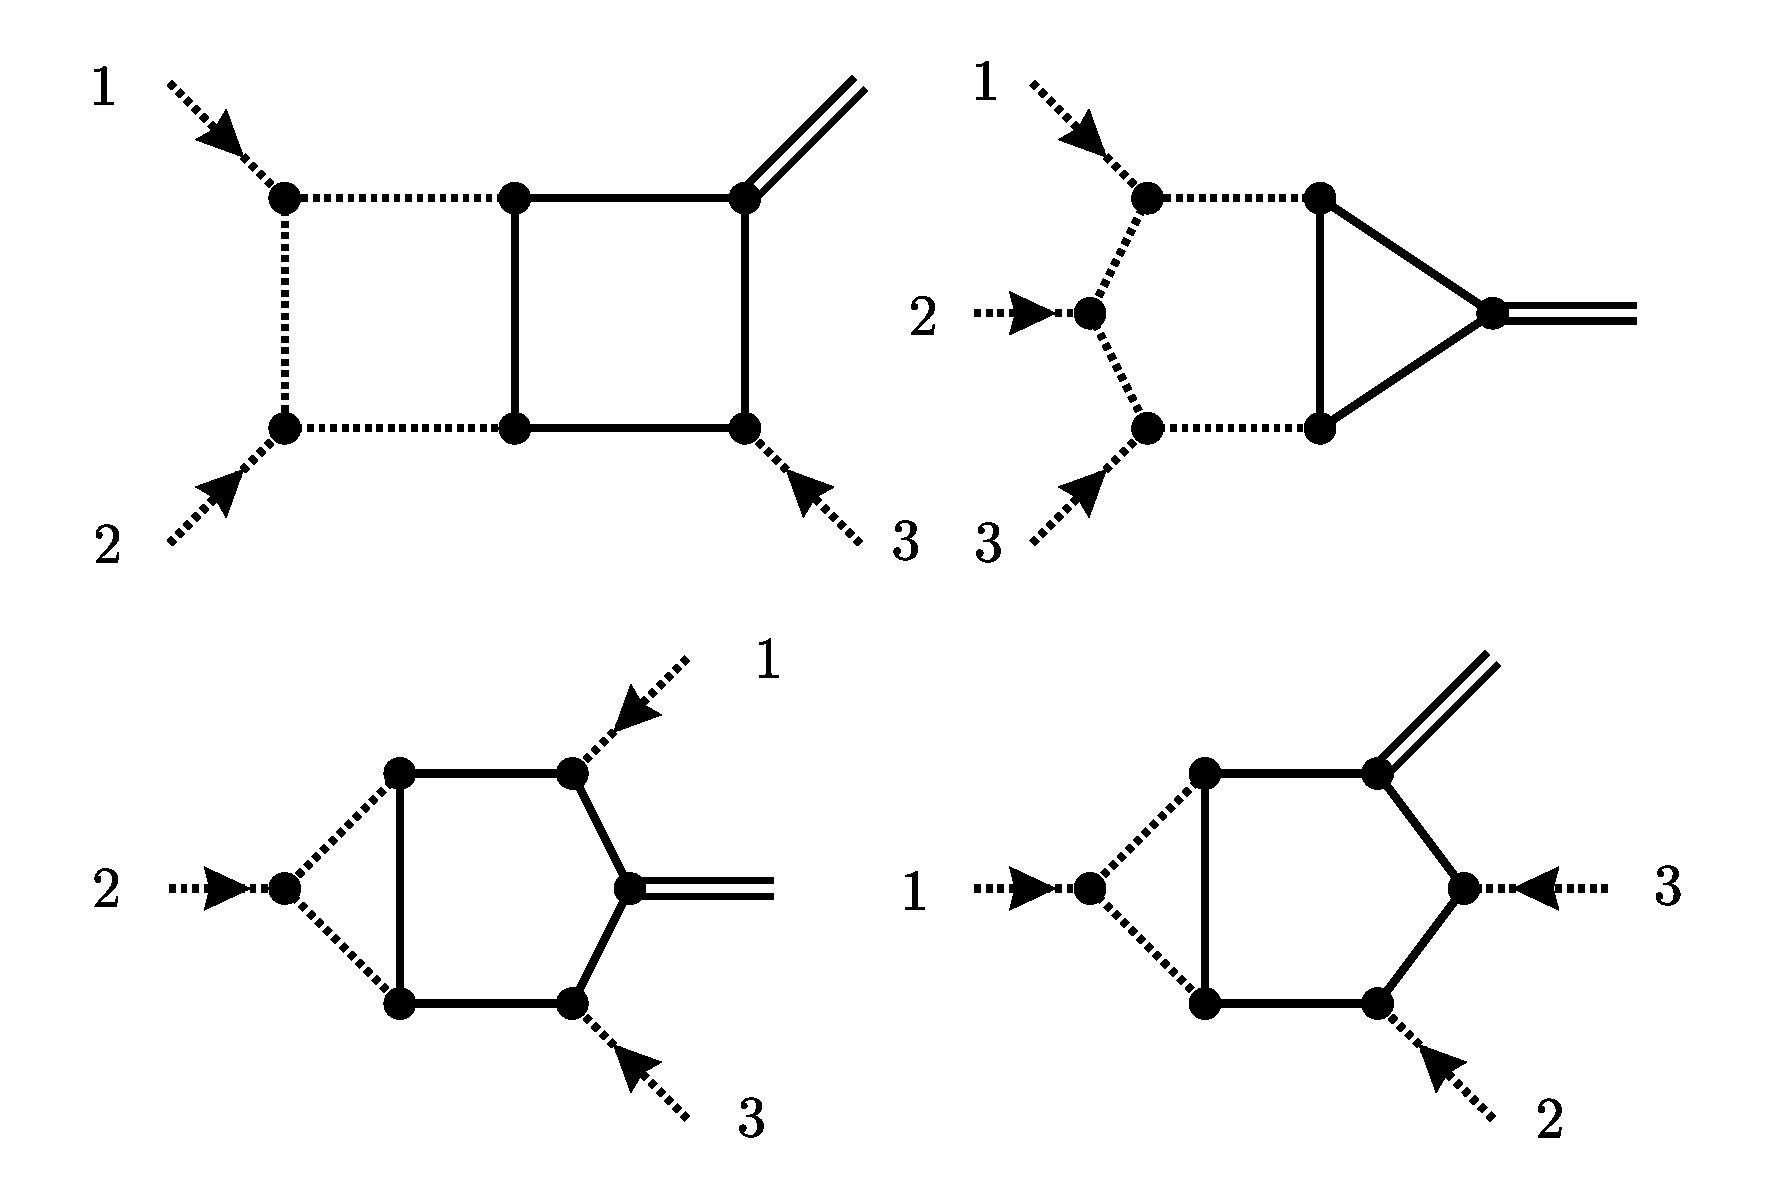
\includegraphics[scale=0.3]{Images/NNLO_Feynman_diagrams/PL1.pdf}
\caption{Graphical representation of the physical sectors embedded in the first integral family (PL1). Dotted lines represent massless propagators, while solid lines have the quark mass in the propagator.} \label{fig:5:PL1}
\end{figure}
\begin{figure}[h]
\centering
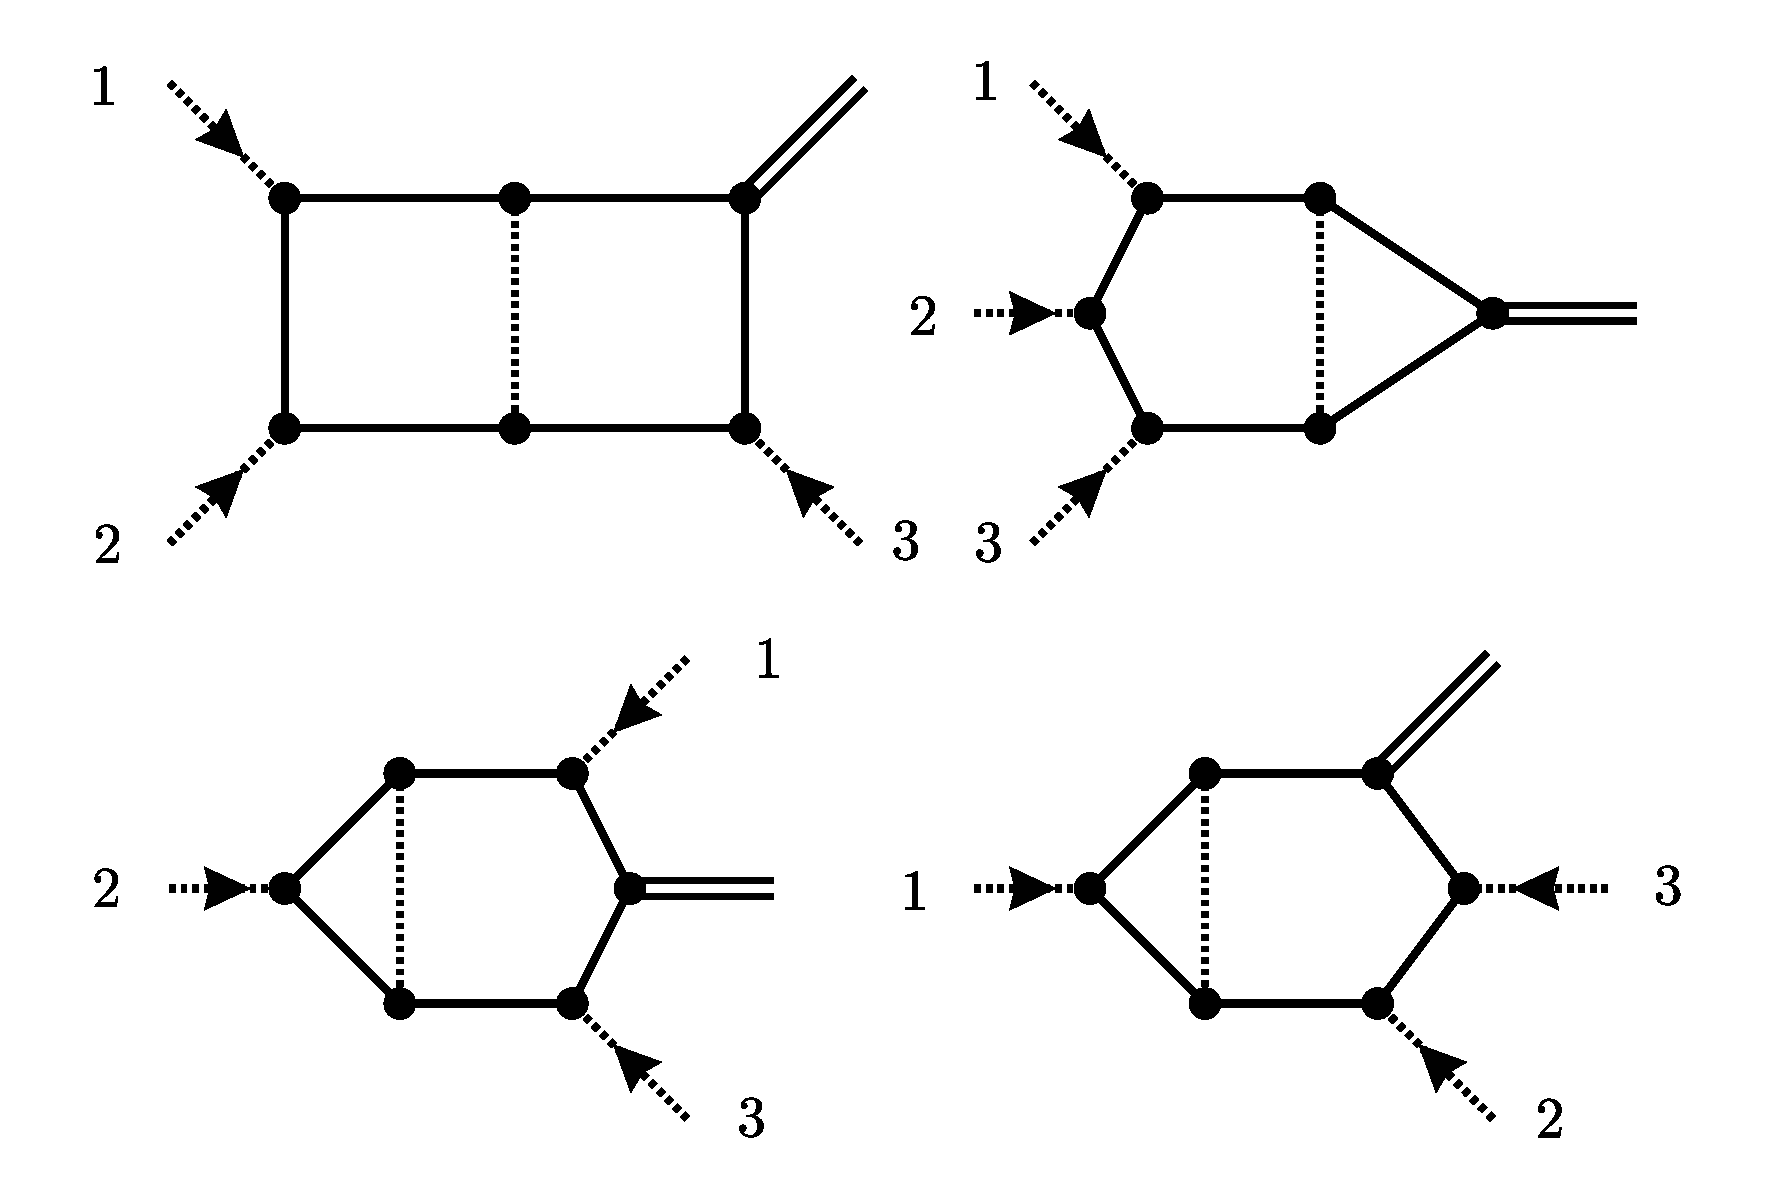
\includegraphics[scale=0.3]{Images/NNLO_Feynman_diagrams/PL2.pdf}
\caption{Same as Fig.~\ref{fig:5:PL1} but for the second integral family (PL2).} \label{fig:5:PL2}
\end{figure}
\begin{figure}[h]
\centering
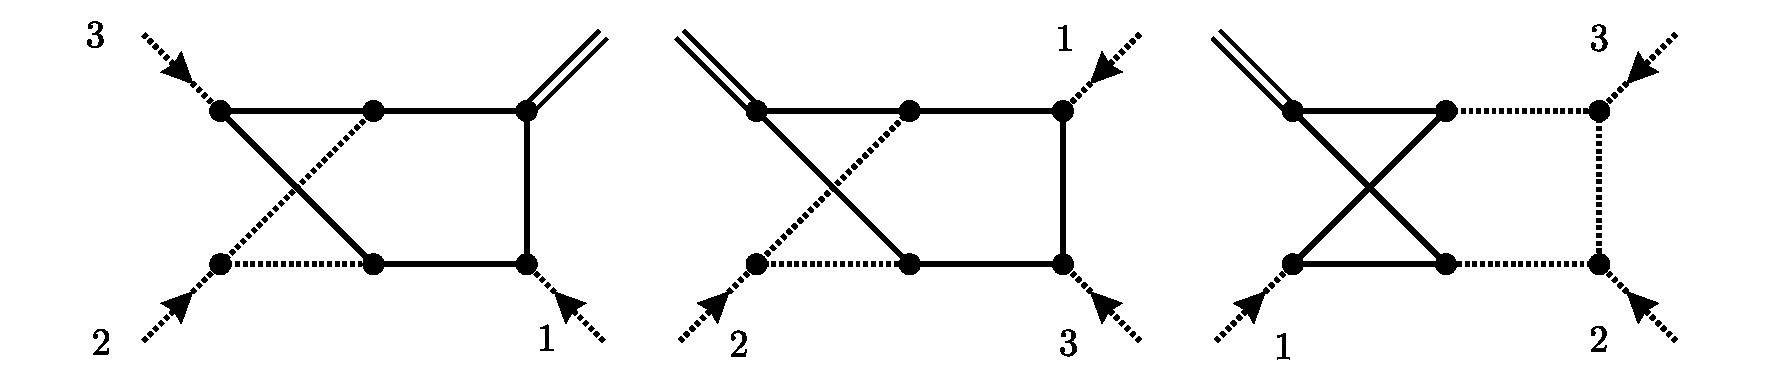
\includegraphics[scale=0.4]{Images/NNLO_Feynman_diagrams/NPL.pdf}
\caption{Same as Fig.~\ref{fig:5:PL1} but for the third non-planar integral family (NPL).} \label{fig:5:NPL}
\end{figure}
For the contributions containing two massive internal quarks, we do not provide the integral families since the two-loop integrals factorize to one-loop integrals.

\textbf{\acs{UV}-Renormalization, \acs{IR}-Subtraction and LSZ-Reduction} \\
So far our analysis was concerned with bare amplitudes regulated in dimensional regularization. The \acs{UV}-poles are eliminated through renormalization of the coupling constant and the quark masses. Following the description in section~\ref{sec:2:cross_sections} we replace the bare coupling constant and masses by their renormalized counterparts and subsequently expand in $\alphas$. The $\alphas^{5/2}$ term is singled out to get the \acs{NNLO} correction to the amplitude. We employ the \MS\ scheme for the $\alphas$, and---for now---the OS scheme for all the quark masses.

To obtain physical amplitudes, we employ the LSZ reduction formula. This means for each external particle, multiplying by the square root of the corresponding LSZ-constant. In dimensional regularization, the LSZ constants only get contributions from heavy fields, since all other contributions render scaleless integrals. This means that the gluon LSZ constants are already non-trivial at one-loop, whereas the quark LSZ constants only gets non-trivial corrections at two-loop, which makes them irrelevant for the calculation at hand. Since bottom-quarks are treated as massless whenever they are not coupling to the Higgs, they do not contribute to the LSZ constants, \ie\ only the top-quark mass enters the LSZ constants.

The remaining poles are of \acs{IR} origin. They would cancel against poles arising during phase-space integration, so we can subtract them already on the amplitude level. We employ the \MS\ scheme and subtract only the divergences predicted by the $\mathbf{Z}$ operator (see for example Ref.~\cite{Czakon:2014oma}).

\textbf{Results for the Contributions with Two Heavy Quarks} \\
Once we performed all the above steps, we separate the contributions which contain two heavy quark loops from the rest of the amplitude. The \acs{IR}-poles, do not receive contributions from heavy internal lines and are therefore irrelevant for this contribution. The LSZ constants of the gluons on the other hand, do contribute. In the coupling renormalization constants, we single out the contributions from the top quark, \ie\ we set the number of fermions to
\begin{equation}
n_f = n_l + n_h
\end{equation}
Here $n_l$ is the number of light quarks, and $n_h$ is the number of heavy quarks. In the 5\acs{FS} we have $n_l = 5$ and $n_h = 1$. The renormalization constant in the \MS\ scheme then reads
\begin{equation}
Z_g = 1 - \frac{\alphas}{4 \pi}  2 \beta_0 \frac{1}{\epsilon} + \BigO{\alphas^2} = 1 + \frac{\alphas}{4 \pi} \frac{1}{\epsilon} \left(- \frac{11}{6} C_A + \frac{2}{3} (n_l + n_h) T_F \right) + \BigO{\alphas^2}.
\end{equation}
To single out the contributions from the top-quark we only take terms proportional to $n_h$ and set $n_h$ to one afterwards. We can then apply the decoupling relations of Eq.~\eqref{eq:4:decoupling} to replace the coupling constant by its decoupled counterpart in the lower order amplitudes\footnote{In the renormalization constants we can simply set $\alphas^{(n_l + n_h)} = \alphas^{(n_l)}$ at this order in perturbation theory.}. We can absorb these terms into the renormalization of the coupling constant, such that we end up with the effective renormalization constant
\begin{equation}
Z_g^{(n_l)} \big \vert_{\propto n_h} = \frac{\alphas}{4 \pi} \frac{2}{3} T_F \left(\frac{1}{\epsilon} - \ln\!\left(\frac{m_t^2}{\mu^2}\right) \right) + \BigO{\alphas^2}.
\end{equation}
This is nothing else than the top-quark contribution to the \acs{OS} coupling renormalization constant. The decoupling constants were specifically introduced to cure the \MS\ scheme from the appearance of non-decoupling effects. In the \acs{OS} scheme this issue does not arise because of the Appelquist-Carrazone theorem (see section~\ref{subsec:4:matching_of_wilson_coefficients}). The equality of the renormalization constants is therefore not accidental.

At one-loop, the top-quark contribution to the renormalization constant is of abelian nature. In \acs{QED}, the Ward identity implies the all order relation $Z_e = Z_3^{-1/2}$. We can therefore conclude, or verify explicitly that the one-loop renormalization constant is also related to the gluon LSZ constant
\begin{equation}
2 Z_g^{(n_l)} \big \vert_{\propto n_h} = - Z_3 + \BigO{\alphas^2}.
\end{equation}
This has the profound effect, that if the external number of gluons is identical to the power of the coupling constant (at lower order), then the contributions exactly cancel. This is for example the case in the $ggg \rightarrow H$ amplitude.

The result for the helicity amplitude of the $ggg \rightarrow H$ amplitude read
\begin{equation}
\begin{split}
&\mathcal{M}^{(1),+++}_{ggg \rightarrow H} \bigg \vert_{2\ \text{masses}} = \frac{1}{\sqrt{2}} \frac{1}{\braket{12}\braket{23} \braket{31}} \bigg \lbrace -  \frac{4 m_t^2 s t u}{(s + t)} \tilde{C}_0\!(u, m_t^2) \bigg [ \tilde{B}\!(m_H^2, m_b^2)  \\
& \hspace{2cm} + \frac{s + t}{u} + 2 \frac{m_b^2}{u} \left( 4 m_b^2 - s - t \right) \tilde{C}_1\!(u, m_H^2, m_b^2) - \frac{4 m_b^2}{s + t} \tilde{B}(u, m_l^2)  \bigg ] \\
& \hspace{5cm} + (s \rightarrow t, t \rightarrow u, u \rightarrow s) + (s \rightarrow u, u \rightarrow t, t \rightarrow s)\bigg \rbrace
\label{eq:5:ggg_ppp}
\end{split}
\end{equation}
%
%
\begin{equation}
\begin{split}
&\mathcal{M}^{(1),-++}_{ggg \rightarrow H} \bigg \vert_{2\, \text{masses}} = -\frac{1}{\sqrt{2}} \frac{[23]^3}{[12][13]} \frac{4 m_t^2 s t }{u(s + t)} \tilde{C}_0\!(u, m_t^2) \bigg [ \tilde{B}\!(m_H^2, m_b^2) \\
& \hspace{2cm} + \frac{s + t}{u} + 2 \frac{m_b^2}{u} \left(4 m_b^2 - s - t\right) \tilde{C}_1\!(u, m_H^2, m_b^2) - \frac{4 m_b^2}{(s + t)} \tilde{B}\!(u, m_b^2) \bigg ]
\label{eq:5:ggg_mpp}
\end{split}
\end{equation}
Where we defined the auxiliary functions\footnote{The functions are closely related to the finite part of the bubble integrals, and the triangle integrals with on-shell, and one off-shell leg. The functions are modified slightly to simplify the expressions, however we keep the standard notation, where $B$ functions indicate bubbles and $C$ functions triangle integrals. The tilde is added to make the distinction from the original integrals more apparent.}
\begin{equation}
\begin{split}
\tilde{B}\!(s, m^2) &\equiv \beta(s, m^2) \log\!\left(- \frac{1 - \beta(s, m^2)}{1 + \beta(s, m^2)} + i 0^+ \right), \\
\tilde{C}_0\!(s, m^2) &\equiv \frac{1}{2 s} \log^2\!\left(- \frac{1 - \beta(s, m^2)}{1 + \beta(s, m^2)} + i 0^+ \right) + \frac{2}{s} \left(\tilde{B}\!(s, m^2) + 2 \right), \\
\tilde{C}_1\!(s_1, s_2, m^2) &\equiv \frac{1}{2} \frac{1}{s_1 - s_2} \left[ \log^2\!\left(-\frac{1 - \beta(s_1, m^2)}{1 + \beta(s_2, m^2)} + i 0^+ \right) - \log^2\!\left(- \frac{1 - \beta(s_2, m^2)}{1 + \beta(s_2, m^2)} + i0^+\right) \right], \\
\text{with} \quad \beta(s, m^2) &\equiv \sqrt{1 - \frac{4 m^2}{s}}.
\label{eq:5:function_definitions}
\end{split}
\end{equation}
All other helicity amplitudes are either related via charge conjugation \eqref{eq:5:parity}, or by relabeling of the external momenta
\begin{equation}
\mathcal{M}_{ggg \rightarrow H}^{+-+} = \mathcal{M}_{ggg \rightarrow H}^{-++} \bigg \vert_{p_1 \leftrightarrow p_2}, \qquad \mathcal{M}_{ggg \rightarrow H}^{++-} = \mathcal{M}_{ggg \rightarrow H}^{-++} \bigg \vert_{p_1 \leftrightarrow p_3}.
\label{eq:5:momentum_exchange}
\end{equation}
Note that the Mandelstam variables are defined in terms of incoming gluon momenta, \ie\
\begin{equation}
s = (p_1 + p_2)^2, \quad t = (p_1 + p_3)^2, \quad u = (p_2 + p_3)^2.
\end{equation}
For the quark channel the result reads
\begin{equation}
\begin{split}
&\mathcal{M}_{\bar{q}q g \rightarrow H}^{(1),-++} \bigg \vert_{2\, \text{masses}} =  \frac{1}{\sqrt{2}} \frac{[13]^2}{[12]}  \frac{4 }{9 (t + u)} \left(5 s + 12 m_t^2 + (3 s + 6 m_t^2) \tilde{B}\!(s, m_t^2) \right)\bigg [\tilde{B}\!(m_H^2, m_b^2) \\
& \hspace{2cm}  + \frac{t + u}{s} + 2 \frac{m_b^2}{s} \left(4m_b^2 - t - u  \right) \tilde{C}_1\!(s, m_H^2, m_b^2) - \frac{4 m_b^2}{t + u}\tilde{B}\!(s, m_b^2) \bigg ].
\label{eq:5:qqg_mpp}
\end{split}
\end{equation}
Once again all other amplitudes can be obtained through a relabeling of the external momenta and charge conjugation. We see that the functional dependence on the Mandelstams is identical in all amplitudes in Eqs.~\eqref{eq:5:ggg_ppp}, \eqref{eq:5:ggg_mpp}, and \eqref{eq:5:qqg_mpp}. This is because the expression is related to the off-shell gluon-Higgs form factor, appearing in all Feynman diagrams of this contribution (see Fig.~\ref{fig:5:real_virtual2}).

\textbf{Contributions With One Heavy Quark} \\
For completeness, we also reproduce the \acs{LO} helicity amplitudes computed in Ref.~\cite{Baur:1989cm}.
\begin{equation}
\begin{split}
& \mathcal{M}_{ggg \rightarrow H}^{(0), +++} = \frac{1}{\sqrt{2}} \frac{16 m^2 stu}{\braket{12}\braket{23}\braket{31}} \bigg \lbrace - 8 \left[ \frac{1}{u t} + \frac{1}{t t_1} + \frac{1}{u u_1} \right] - \frac{8}{s} \left[ \frac{2 s + t}{u_1^2} B_1(u) + \frac{2 s + u}{t_1^2} B_1(t) \right] \\
& \qquad - \frac{2 (s - 4 m^2)}{stu} \left[ s_1 C_1(s) + (u - s) C_1(t) + (t - s) C_1(u) \right] - 16 m^2 \left[ \frac{1}{t t_1} C_1(t) + \frac{1}{u u_1} C_1(u) \right] \\
& \qquad + \frac{8 m^2}{s} D(u, t) + \frac{s - 4 m^2}{s t u} \left[ s t D(s, t) + u s D(u, s) - u t D(u, t) \right] - \frac{4}{s^2} E(u, t) \bigg \rbrace
\end{split}
\end{equation}
%
%
\begin{equation}
\begin{split}
& \mathcal{M}_{ggg \rightarrow H}^{(0), -++} = \frac{1}{\sqrt{2}} \frac{[23]^3}{[12][13]} \frac{16 m^2 s t}{u} \bigg \lbrace \frac{8 m_H^2}{s t u} + \frac{2 (m_H^2 - 4 m^2)}{stu} \left[ s_1 C_1(s) + u_1 C_1(u) + t_1 C_1(t) \right] \\
&\qquad - \frac{m_H^2 - 4 m^2}{stu} \left[ s t D(s, t) + u s D(u, s) + u t D(u, t) \right] \bigg \rbrace
\end{split}
\end{equation}
%
%
\begin{equation}
\mathcal{M}_{\bar{q} q \rightarrow H}^{(0), -++} = \frac{1}{\sqrt{2}} \frac{[13]^2}{[12]} \frac{m^2}{s_1} \left[ 2 + 2 \frac{s}{s_1} B_1(s) + \left(4 m^2 - u - t \right) C_1(s) \right]
\end{equation}
Here $m$ is the internal quark mass and we defined
\begin{equation}
s_1 = s - m_H^2, \quad t_1 = t - m_H^2, \quad u_1 = u - m_H^2.
\end{equation}
The appearing functions are directly linked to standard Feynman integrals which we provide in Appendix~\ref{app:2}.
\todo{Check numerically}

Although there is one less scale in the contributions with only one quark mass, the two-loop amplitudes are a lot more complex because the integrals do no longer factorize. Instead of attempting to solve the remaining integrals analytically, we followed a numerical approach, where the amplitudes are evaluated at fixed phase-space points. These points can then be used as grid points for interpolations during the phase-space integration. For the numerical evaluation of the master integrals we follow the strategy outlined in Ref.~\cite{Czakon:2021yub}, which itself is based on methods presented in Ref.~\cite{Czakon:2015exa}. The general idea is to derive a system of differential equation for each integral family, find suitable boundary conditions analytically, and then solve the differential equations numerically.

The amplitude is a function of four variables, \eg\ $s, t, u$ and the quark mass $m$. The Higgs mass is not a free parameter since it can be expressed as a sum over the Mandelstams. We can however simply factor our one scale, say the collision scale $s$ to make everything dimensionless, and we are left with only three. We choose to parametrize the amplitude in terms of the dimensionless variables
\begin{equation}
z \equiv - \frac{t + u}{s}, \quad \lambda \equiv \frac{t}{t + u}, \quad x \equiv \frac{m^2}{s} = \frac{m^2}{m_H^2} (1 - z).
\label{eq:5:physical_parameter_space}
\end{equation}
These variables are advantageous because they parametrize soft and collinear limits. Indeed, soft limits are described with $z \rightarrow 0$, whereas the collinear limits are captured by $\lambda \rightarrow 0$ for the $t$-collinear and $\lambda \rightarrow 1$ for $u$-collinear. Furthermore, $z$ and $\lambda$ are bounded by
\begin{equation}
0 \le z \le 1, \quad 0 \le \lambda \le 1, \quad \text{and} \quad 0 \le x
\end{equation}
for physical production kinematics.

To apply the method of differential equations, we need to apply derivatives with respect to our variables, but the master integrals are functions of the external momenta. We can apply the chain rule to relate the derivatives
\begin{alignat*}{2}
\refstepcounter{equation}
&\left(z \frac{\partial }{\partial z} \right) &&= \left(t \frac{\partial }{ \partial t} \right) + \left( u \frac{\partial}{ \partial u} \right) + \frac{t + u}{s + t + u} \left(x \frac{\partial}{ \partial x} \right) \\
& &&= \left(p_3^\mu \frac{\partial}{\partial p_3^\mu} \right) - \frac{z}{1 - z} \left(x \frac{\partial }{\partial x} \right), \tag{\theequation} \\
\refstepcounter{equation}
& \left(\lambda \frac{\partial}{\partial \lambda}\right) && = \left(t \frac{\partial}{\partial t} \right) - \frac{\lambda}{1 - \lambda} \left(u \frac{\partial}{\partial u} \right) \\
& &&= \frac{1}{2} \left( \left(p_1^\mu \frac{\partial}{\partial p_1^\mu} \right) - \left(p_2^\mu \frac{\partial}{\partial p_2^\mu} \right) + (1 - 2 \lambda) \left(p_3^\mu \frac{\partial}{\partial p_3^\mu} \right)\right).  \tag{\theequation}
\end{alignat*}
The derivative with respect to $x$ remains unchanged. One can now proceed to apply the differential operators onto the master integrals. The derivatives result in new integrals, which we can relate to our master integrals through the repeated use of \acs{IBP}s.

We found that it is advantageous shift almost all the appearing master integrals from $d = 4 - 2 \epsilon$ to $d + 2$ dimensions, by application of \textit{dimension-shift relations} (see Ref.~\cite{Weinzierl:2022eaz} for a comprehensive introduction). This way, all spurious poles of the top-level sector are removed, and the integrals must only be computed up to $\epsilon^0$. As a byproduct, we found that the coefficients in front of the master integrals are significantly reduced in complexity.

In order to solve the differential equation, we need to find suitable boundary conditions. Since the \acs{HTL} has already been extensively studied, it suggests itself to use it as boundary conditions. To this end, we expand the integrals in the limit of a large internal mass $m, x \rightarrow \infty$ by means of the \textit{large mass expansion} (see Ref.~\cite{Smirnov:2002pj} for a comprehensive introduction). It allows expanding integrals in the limit of large masses already at the integral level, \ie\ the remaining integrals are devoid of the large mass. The expansion is implemented in the workflow of \texttt{DiaGen/IdSolver}. The only required integrals are massless four-point functions and vacuum integrals which can be found in the appendix of Ref.~\cite{Niggetiedt:2023ywb}.

The solutions found at the boundary $x \rightarrow \infty$ can now be transported to the physical plane, \ie\ to finite quark masses by solving the differential equation in the $x$-direction. This strategy is illustrated in Fig.~\ref{fig:5:integration3D}.
\begin{figure}[h]
\centering
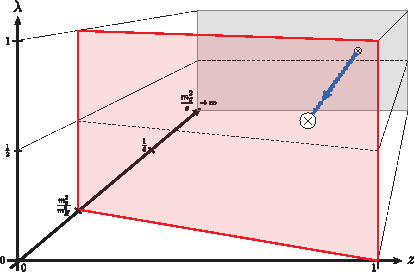
\includegraphics[width=\figurewidth]{Images/integration3D_no_threshold.pdf}
\caption{Graphical illustration of the parameter space and the strategy for transporting the boundary conditions at $x \rightarrow \infty$ to the physical plane shown in red. Figure taken (with slight modification) from Ref.~\cite{Niggetiedt:2023ywb}.}
\label{fig:5:integration3D}
\end{figure}
The differential equation is solved numerically using the \textit{Bulirsch-Stoer algorithm}. Since we are working within the physical parameter space defined by Eq.~\eqref{eq:5:physical_parameter_space}, we can no longer relate the various matrix elements by means of crossing relations Eq.~\eqref{eq:5:momentum_exchange}. We will therefore have to switch to a physical momentum configuration and compute all matrix elements\footnote{The helicities are assigned to the partons in the order they appear in the corresponding process,\ie \ the first helicity belongs to the first appearing parton, the second to the second, and the third to the third.}
\begin{equation}
\begin{split}
&\mathcal{M}_{gg \rightarrow H g}^{+++}, \mathcal{M}_{gg \rightarrow g H }^{-++}, \mathcal{M}_{gg \rightarrow gH}^{+-+}, \mathcal{M}_{gg \rightarrow gH}^{++-}, \mathcal{M}_{gg \rightarrow gH }^{+++}, \\
&\mathcal{M}_{\bar{q} q \rightarrow gH }^{-++}, \mathcal{M}_{\bar{q} q \rightarrow gH }^{+-+}, \mathcal{M}_{g\bar{q} \rightarrow \bar{q}H}^{+-+}, \mathcal{M}_{g\bar{q} \rightarrow \bar{q}H}^{++-}, \mathcal{M}_{qg \rightarrow q H}^{++-}, \mathcal{M}_{qg \rightarrow q H}^{-++}
\end{split}
\end{equation}
individually. Notice that we can still apply the charge conjugation identity in Eq.~\eqref{eq:5:parity} if we first pull out the spinor-helicity factors. Nevertheless, the exchange of the first two momenta does not take us out of the physical parameter space and hence the crossing symmetry (followed by charge conjugation) can still be exploited.
\begin{alignat}{2}
& |\mathcal{M}_{gg \rightarrow g H}^{\lambda_1 \lambda_2 \lambda_3} |^2(\lambda, z, x) &&= |\mathcal{M}_{gg \rightarrow g H}^{\lambda_2 \lambda_1 \lambda_3}|^2 (1 - \lambda, z, x), \label{eq:5:symmetry_1} \\
& |\mathcal{M}_{\bar{q}q \rightarrow g H}^{\lambda_1 \lambda_2 \lambda_3}|^2 (\lambda , z, x) &&= |\mathcal{M}_{\bar{q} q \rightarrow g H}^{\lambda_2 \lambda_1 \lambda_3}|^2 (1 - \lambda , z, x),\label{eq:5:symmetry_2} \\
& |\mathcal{M}_{qg \rightarrow qH}^{\lambda_1 \lambda_2 \lambda_3}|^2 (\lambda, z, x) &&= |\mathcal{M}_{g \bar{q} \rightarrow \bar{q} H}^{\lambda_2 \lambda_1 \lambda_3}|^2 (1 - \lambda, z, x). \label{eq:5:symmetry_3}
\end{alignat}
We relate the squared amplitudes to avoid phase factors arising from the spinor-helicity factors. The physical parameter space is therefore effectively cut in half. Consequently, we only have to solve the amplitude for $1/2 \le \lambda \le 1$ and can infer the remaining space with these symmetry relations.

We therefore choose initial conditions which are just above the symmetry line $\lambda = 1/2$, and then sample different values in $z$. The solutions of the differential equation in $x$ for these samples then serve as initial conditions for the differential equation in $\lambda$. This is illustrated in Fig.~\ref{fig:5:integration2D}.
\begin{figure}
\centering
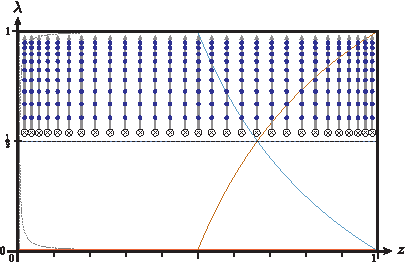
\includegraphics[width=\figurewidth]{Images/integration_Z_LA_with_poles_mb2_with_contour.pdf}
\caption{Illustration of the physical plane (shown in red in Fig.~\ref{fig:5:integration3D}) for a bottom quark with a mass ratio of $m_b^2/m_H^2 = 1/684$. The colored thin lines indicate poles of the differential equation in $\lambda$. The circled crosses with the errors indicate the boundary condition for the differential equation in $\lambda$ and the path along which the differential equation is solved. The integration paths are not to scale and are for illustrative purposes only.}
\label{fig:5:integration2D}
\end{figure}
At $z \rightarrow 0$, we encounter a soft divergence. These divergences will cancel in the end, but it is therefore important to map out this parameter space with particular care. We therefore sample $z$ logarithmically. Furthermore, for $z \rightarrow 1$ the poles of the differential equation are very close together. This once again causes large cancellations. To avoid mismodelling the amplitudes in these regions of the parameter space we therefore also sample more points close to this boundary. In the end we sample around $1000$ values of $z$, ranging from $10^{-4}$ to $1 - 10^{-4}$.

The poles of the differential equation in $\lambda$ are dealt with via a contour deformation in the complex plane. Once again we sample $\lambda$ logarithmically, such that we obtain more points towards the \acs{IR}-sensitive $\lambda \rightarrow 1$ region. In total, we sample around $500$ points, yielding dense grid of the physical plane of around $10^6$ grid points.

Around the \acs{IR} sensitive regions $z \rightarrow 0$ and $\lambda \rightarrow 0, 1$, the amplitudes are dominated by the singularities $1/z$ and $1/\sqrt{\lambda}$, a contribution which will eventually cancel against other \acs{IR} divergences. On the other hand, the dominance of the singularity will negatively impact the precision of the interpolation for the non-divergent terms. We would therefore like to subtract the \acs{IR}-divergences before performing the interpolation. It is well known, that the leading \acs{IR} behavior factorizes from the amplitude. Consider for example, the limit of two almost collinear outgoing partons with momenta
\begin{equation}
p_1^\mu = z_1 p^\mu + k_\perp^\mu - \frac{k_\perp^2}{z_1} \frac{n^\mu}{2 p \cdot n}, \qquad p_2^\mu = (1 - z_1) p^\mu - k_\perp - \frac{k_\perp^2}{1 - z} \frac{n^\mu}{2 p \cdot n},
\end{equation}
where $k_\perp \cdot p = k_\perp \cdot n = 0$, and $p$ and $n$ are on-shell ($p^2 = n^2 = 0$). Further $p$ and $n$ are not collinear, \ie\ $p \cdot n \sim \BigO{p^0 n^0}$. The collinear limit is therefore parametrized by $k_\perp \rightarrow 0$. Then the leading power behavior of the one-loop averaged squared matrix element is given by
\begin{equation}
\begin{split}
2 \text{Re} &\overline{\braket{\mathcal{M}_{a_1 a_2,\cdots}^{(0)} (p_1, p_2, \ldots)| \mathcal{M}_{a_1 a_2,\cdots}^{(1)} (p_1, p_2, \ldots)}} \simeq \\
& \quad 4 \pi \alphas \frac{1}{p_1 \cdot p_2} \left[ \braket{P^{(0)}_{a_1 a_2}(z_1)} \times 2 \text{Re} \overline{\braket{\mathcal{M}_{a,\cdots}^{(0)} (p, \ldots)| \mathcal{M}_{a,\cdots}^{(1)} (p, \ldots)}} \right. \\
&\hspace{3cm} \left. + \frac{\alphas}{4 \pi} \braket{P^{(1)}_{a_1 a_2}(z_1)} \overline{\braket{\mathcal{M}_{a,\cdots}^{(0)} (p, \ldots)| \mathcal{M}_{a,\cdots}^{(0)} (p, \ldots)}} \right].
\end{split}
\label{eq:5:collinear_limit}
\end{equation}
Here $a_1$ and $a_2$ denote the flavor of the respective parton, while the flavor $a$ is set by flavor conservation. $\braket{P^{(0,1)}_{a_1 a_2}(z_1)}$ are the tree-level and one-loop averaged splitting functions. For reasons that will be explained below, the exact structure of the one-loop splitting functions is of no concern to us. The tree-level averaged splitting functions in four dimensions read
\begin{equation}
\begin{split}
\braket{P_{gg}^{(0)}(z_1)} &= 2 C_A \left( \frac{z_1}{1 - z_1} + \frac{1 - z_1}{z_1} + z_1 (1 - z_1) \right), \\
\braket{P_{q \bar{q}}^{(0)} (z_1)} = \braket{P_{\bar{q}q}^{(0)} (z_1)} &= T_F \left(1 - 2 z_1 (1 - z_1) \right), \\
\braket{P_{qg}^{(0)}(z_1)} = \braket{P_{\bar{q}g}^{(0)}(z_1)} &= C_F \frac{1 + z_1^2}{1 - z_1} \\
\braket{P^{(0)}_{gq}(z_1)} = \braket{P_{g\bar{q}}^{(0)}(z)} &= \braket{P_{qg}^{(0)} (1 - z)}.
\end{split}
\end{equation}
Initial state collinear divergences can be recovered by replacing $p_2 \rightarrow - p_2$ as well as $P_{a_1 a_2} \rightarrow (-1)^{2 s_a + 2 s_{a_1}} P_{a_1 a_2}$, where $s_a$ and $s_{a_1}$ are the spins of the respective partons.

Likewise, in the limit where one of the external gluons becomes soft, $q \rightarrow 0$, the factorization of the one-loop squared amplitude with external partons reads
\begin{equation}
\begin{split}
&2 \text{Re} \braket{\mathcal{M}^{(0)}_{g,a_1,\cdots} (q, p_1, \ldots)|\mathcal{M}^{(1)}_{g,a_1,\cdots} (q, p_1, \ldots)} \simeq \\
&\qquad - 4 \pi \alphas \bigg \lbrace \sum_{(i,j)} \left( \mathcal{S}_{ij}(q) - \mathcal{S}_{ii}(q) \right) 2 \text{Re} \braket{\mathcal{M}^{(0)}_{a_1,\cdots} ( p_1, \ldots)| \mathbf{T}_i \cdot \mathbf{T}_j|\mathcal{M}^{(1)}_{a_1,\cdots} (p_1, \ldots)}  \\
& \hspace{3cm} + \frac{\alphas}{4 \pi} \bigg [ \sum_{(i,j)} \left( \mathcal{S}_{ij}(q) - \mathcal{S}_{ii}(q) \right) R_{ij} \braket{\mathcal{M}^{(0)}_{a_1,\cdots} ( p_1, \ldots)| \mathbf{T}_i \cdot \mathbf{T}_j|\mathcal{M}^{(0)}_{a_1,\cdots} (p_1, \ldots)}  \\
& \hspace{4cm}  - 4 \pi \sum_{(i,j,k)} \mathcal{S}_{ik} (q) I_{ij} \braket{\mathcal{M}^{(0)}_{a_1,\cdots} ( p_1, \ldots)| f^{abc} \mathbf{T}_i^a \mathbf{T}_j^b \mathbf{T}_k^c|\mathcal{M}^{(1)}_{a_1,\cdots} (p_1, \ldots)} \bigg ] \bigg \rbrace
\end{split}
\label{eq:5:soft_limit}
\end{equation}
The sums run over distinct parton indices. $\mathbf{T}_i$ denotes the color operator of the $i$-th particle, \ie\ it is the generator of the \SU{3} group in the representation of that particle: fundamental for quarks, complex-conjugated for anti-quarks, adjoint for gluons and trivial for colorless particles. Once again, the exact structure of the one-loop coefficients $I_{ij}, R_{ij}$ is irrelevant to us (see Ref.~\cite{Czakon:2015exa} for a definition). The eikonal factor is given by
\begin{equation}
\mathcal{S}_{ij}(q) = \frac{p_i \cdot p_j}{(p_i \cdot q) (p_j \cdot q)}.
\end{equation}

We claim that the regulated averaged squared amplitudes\footnote{\todo{Notice the different signs infront of the splitting functions compared to Ref.~\cite{Czakon:2024ywb}.}}
\begin{equation}
\begin{split}
&\overline{\braket{\mathcal{M}^{(0)}_{gg\rightarrow gH} | \mathcal{M}^{(1)}_{gg \rightarrow gH}}} \vert_\text{regulated} \equiv  \overline{\braket{\mathcal{M}^{(0)}_{gg\rightarrow gH} | \mathcal{M}^{(1)}_{gg \rightarrow gH}}} -  \overline{\braket{\mathcal{M}^{(0), \text{rHTL}}_{gg\rightarrow gH} | \mathcal{M}^{(1), \text{rHTL}}_{gg \rightarrow gH}}} \\
& \quad - \overline{\braket{\mathcal{M}^{(0)}_{gg \rightarrow H} | \mathcal{M}^{(1)}_{gg \rightarrow H} - \mathcal{M}^{(1), \text{rHTL}}_{gg \rightarrow H}} }  \times \begin{cases} \frac{8 \pi \alphas}{t} \braket{P_{gg}^{(0)} \!\left(\frac{s}{s + u} \right)} \quad &\text{if } |t| < |u| \\
\frac{8 \pi \alphas}{u} \braket{P_{gg}^{(0)} \!\left(\frac{s}{s + t} \right)} \quad &\text{if } |u| < |t|
\end{cases}, \\[0.2cm]
& \overline{\braket{\mathcal{M}^{(0)}_{qg\rightarrow qH} | \mathcal{M}^{(1)}_{qg \rightarrow qH}}} \vert_\text{regulated} \equiv  \overline{\braket{\mathcal{M}^{(0)}_{qg\rightarrow qH} | \mathcal{M}^{(1)}_{qg \rightarrow qH}}} -  \overline{\braket{\mathcal{M}^{(0), \text{rHTL}}_{qg\rightarrow qH} | \mathcal{M}^{(1), \text{rHTL}}_{qg \rightarrow qH}}} \\
& \quad + \overline{\braket{\mathcal{M}^{(0)}_{gg \rightarrow H} | \mathcal{M}^{(1)}_{gg \rightarrow H} - \mathcal{M}^{(1), \text{rHTL}}_{gg \rightarrow H}}}  \times
\frac{8 \pi \alphas}{t} \braket{P_{q\bar{q}}^{(0)} \!\left(\frac{s}{s + u} \right)}, \\[0.2cm]
&\overline{\braket{\mathcal{M}^{(0)}_{q\bar{q}\rightarrow gH} | \mathcal{M}^{(1)}_{q \bar{q} \rightarrow gH}}} \vert_\text{regulated} \equiv  \overline{\braket{\mathcal{M}^{(0)}_{q \bar{q}\rightarrow gH} | \mathcal{M}^{(1)}_{q\bar{q} \rightarrow gH}}} -  \overline{\braket{\mathcal{M}^{(0), \text{rHTL}}_{q \bar{q} \rightarrow gH} | \mathcal{M}^{(1), \text{rHTL}}_{q \bar{q} \rightarrow gH}}}, \\
\end{split}
\label{eq:IR_regulation}
\end{equation}
are free of \acs{IR} divergences. The averaged splitting functions are
\begin{equation}
\braket{P_{gg}^{(0)}(z)} = 2 C_A \left( \frac{z}{1 - z} + \frac{1 - z}{z} + z (1 - z) \right) \quad \text{and} \quad \braket{P_{q \bar{q}}^{(0)}(z)} = T_F \left(1 - 2 z (1 - z) \right).
\end{equation}

By subtracting the amplitude in the \acs{rHTL} we are eliminating all infrared divergences coming from one-loop splitting functions or soft functions in Eqs.~\eqref{eq:5:collinear_limit} and\ \eqref{eq:5:soft_limit}. These functions only act upon the difference of the \acs{LO} Higgs-gluon form factor in \acs{QCD} and in the \acs{rHTL}. But this difference is zero by definition of the \acs{rHTL}. Notice that the factor used for rescaling the cross section in the \acs{HTL} for the interference contributions is now defined in terms of
\begin{equation}
r^\mathrm{LO}_{t \times b} = \frac{\hat{\sigma}_{t \times b}^{\mathrm{LO}}}{\hat{\sigma}_{t \times b}^{\mathrm{LO}, \mathrm{rHTL}}},
\end{equation}
which for on-shell masses yields approximately $-0.129$. In contrast to the rescaling factor for the pure top-quark contribution, this rescaling factor has no direct phenomenological relevance, in the sense that it can incorporate finite quark mass effects, and is used only as a computational trick.

After subtraction of the \acs{rHTL} squared amplitudes, the difference still exhibits divergences from tree-level splitting and soft functions. For the $gg \longrightarrow g H$ amplitude the divergence can be handled by subtracting
\begin{equation}
\overline{\braket{\mathcal{M}^{(0)}_{gg \rightarrow H} | \mathcal{M}^{(1)}_{gg \rightarrow H} - \mathcal{M}^{(1), \text{rHTL}}_{gg \rightarrow H}}}  \times \begin{cases} \frac{8 \pi \alphas}{t} \braket{P_{gg}^{(0)} \!\left(\frac{s}{s + u} \right)} \quad &\text{if } |t| < |u| \\
\frac{8 \pi \alphas}{u} \braket{P_{gg}^{(0)} \!\left(\frac{s}{s + t} \right)} \quad &\text{if } |u| < |t|
\end{cases}
\label{eq:5:gggH_limit}
\end{equation}
from the difference. To see this, let us first consider the $t$-collinear limit, \ie\ $p_1 \cdot p_3 \rightarrow 0$. We can choose the anti-collinear direction to be along $p_2$ and then determine\footnote{Note that $z$ is only unique up to power corrections.}
\begin{equation}
z_1 = \frac{p_1 \cdot p_2}{p_1 \cdot p_2 - p_3 \cdot p_2} = \frac{s}{s - u}.
\end{equation}
Hence, Eq.~\eqref{eq:5:gggH_limit} has exactly the structure required from a collinear limit \eqref{eq:5:collinear_limit}. The $u$-collinear limit works analogously. The soft limit, where $t$ and $u$ tend to zero, we can expand the splitting functions and get
\begin{equation}
\eqref{eq:5:gggH_limit} \rightarrow \overline{\braket{\mathcal{M}^{(0)}_{gg \rightarrow H} | \mathcal{M}^{(1)}_{gg \rightarrow H} - \mathcal{M}^{(1), \text{rHTL}}_{gg \rightarrow H}}}  \times  \frac{8 \pi \alphas}{t} 2 C_A \frac{s}{u}.
\end{equation}
Remembering that the Higgs-gluon form factor was diagonal in color-space, \ie\ proportional to $\delta^{c_1 c_2}$, we see that this is exactly the soft divergence predicted by Eq.~\eqref{eq:5:soft_limit}.

Lacking a final state gluon, the $q g$-channel can not develop a soft divergence. The initial state collinear divergence is subtracted with the corresponding splitting functions analogous to the $gg$ channel. The different sign comes from the splitting function, which generates a minus sign if a fermion is crossed to the initial state.

Lastly, after subtraction of the squared amplitude of the \acs{rHTL} the $q \bar{q}$-channel does not exhibit any \acs{IR} singularity, due to the lack of available Born processes.

In Fig.~\ref{fig:5:RV_tOSbOS} we present the results for the top-bottom interference contribution to the amplitudes, while Fig.~\ref{fig:5:RV_tOStOS} shows the results for the pure-top-quark contribution.
\begin{figure}[h]
  \begin{minipage}[t]{0.49\textwidth}
  \centering
  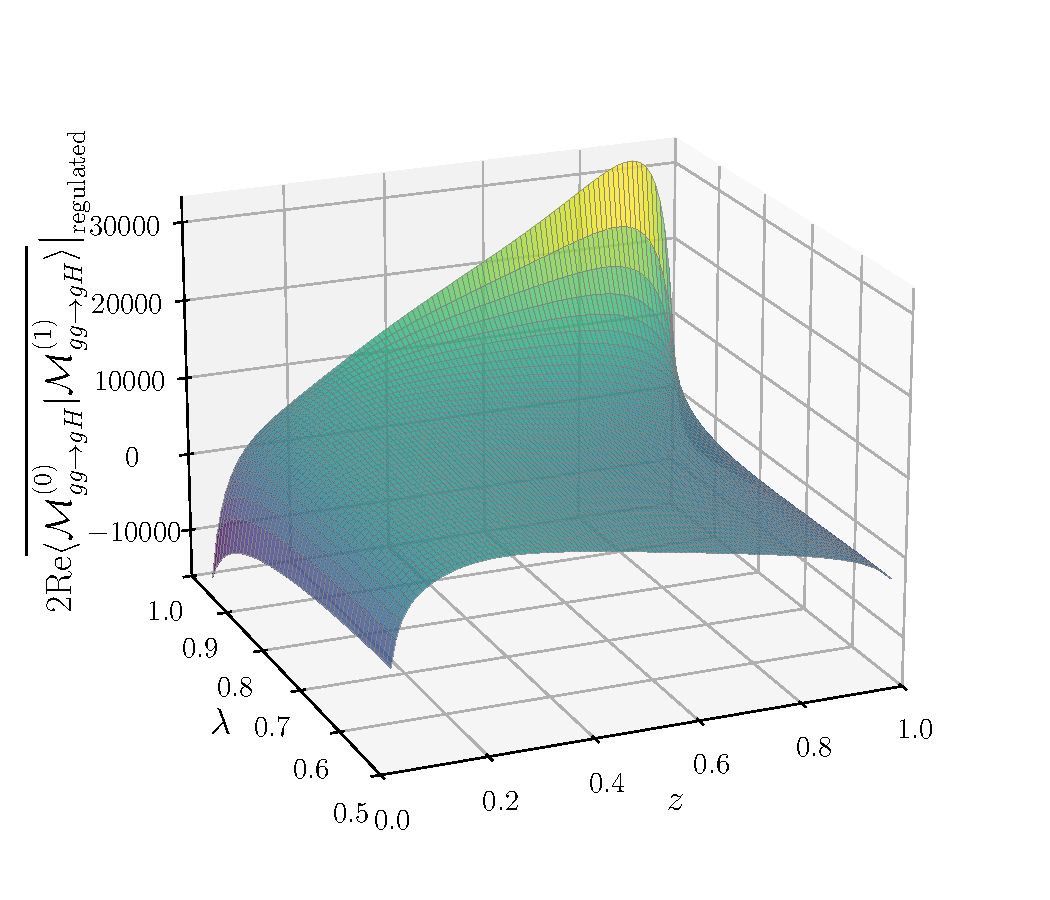
\includegraphics[width=\textwidth]{Images/RV_amplitudes/tOSbOS_gg.pdf}
  %\captionof{figure}{gg}
  %\label{fig:2:PDF}
  \end{minipage}
  \begin{minipage}[t]{0.49\textwidth}
  \centering
  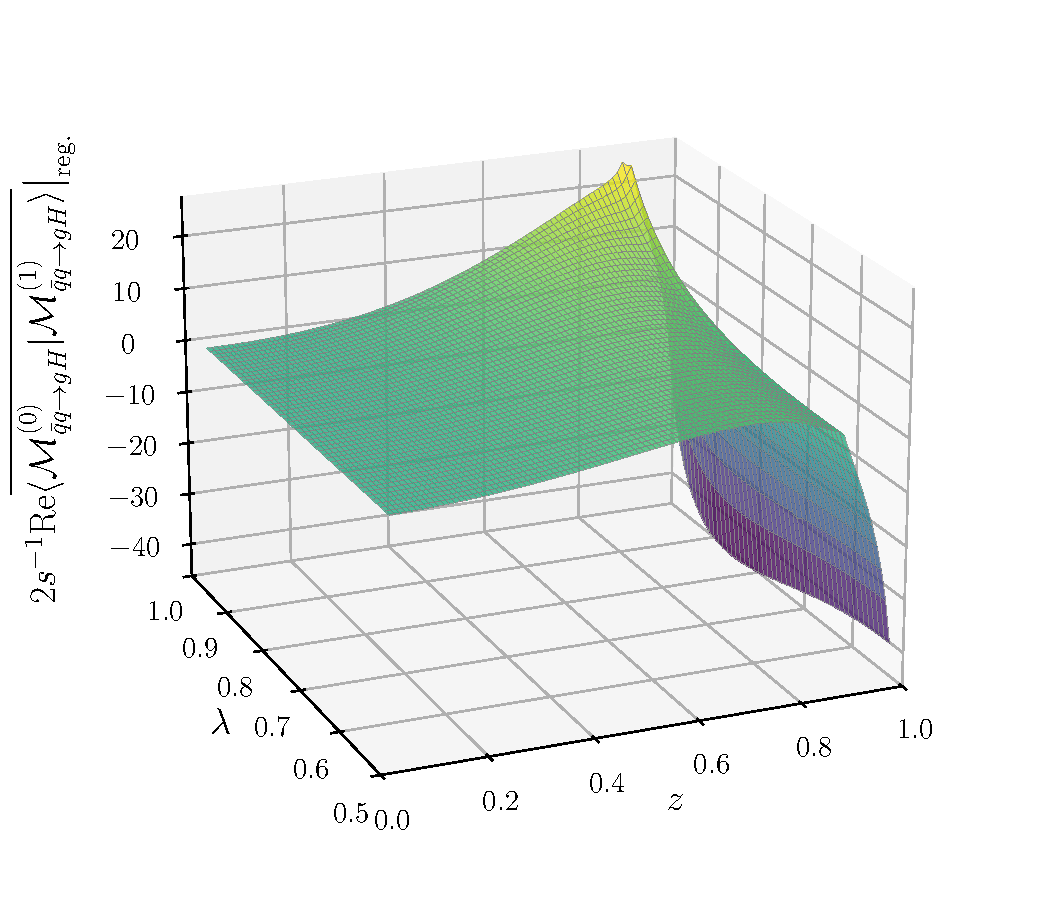
\includegraphics[width=\textwidth]{Images/RV_amplitudes/tOSbOS_qBq.pdf}
  %\captionof{figure}{}
  %\label{fig:2:luminosity}
  \end{minipage}
  \begin{minipage}[t]{0.49\textwidth}
  \centering
  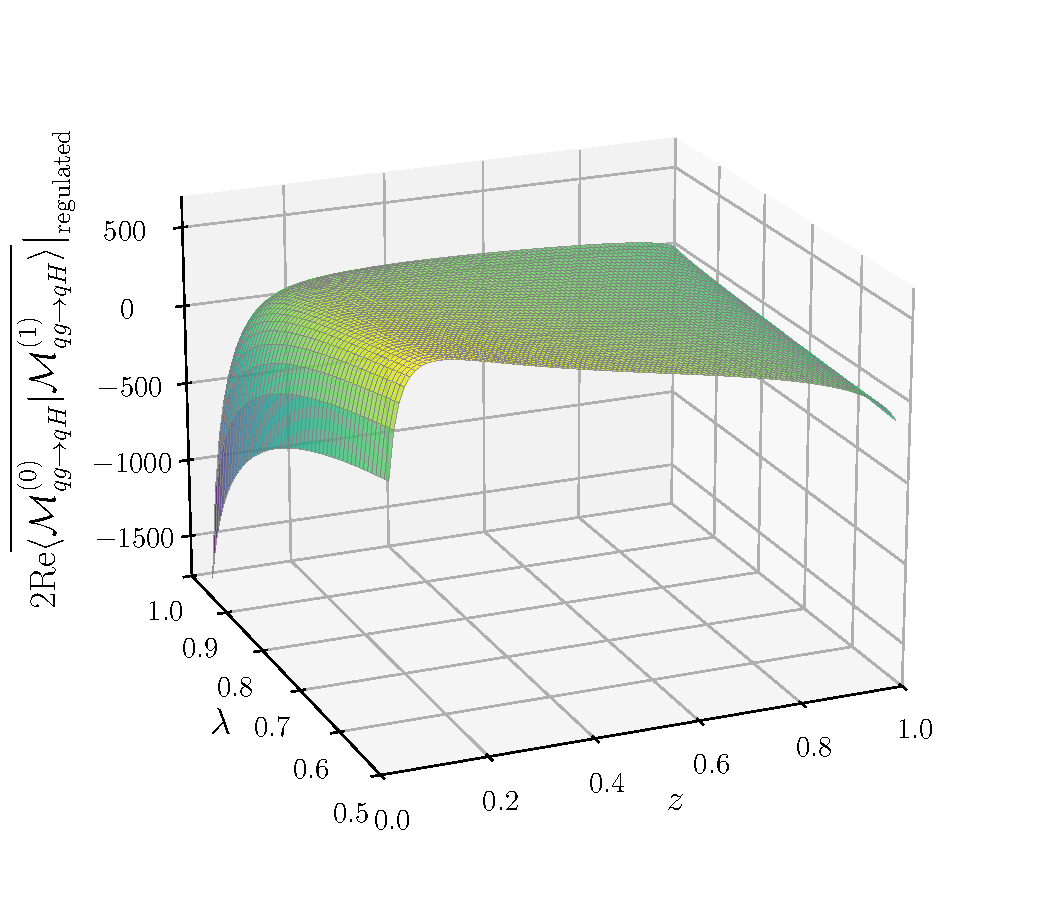
\includegraphics[width=\textwidth]{Images/RV_amplitudes/tOSbOS_qg.pdf}
  %\captionof{figure}{gg}
  %\label{fig:2:PDF}
  \end{minipage}
  \begin{minipage}[t]{0.49\textwidth}
  \centering
  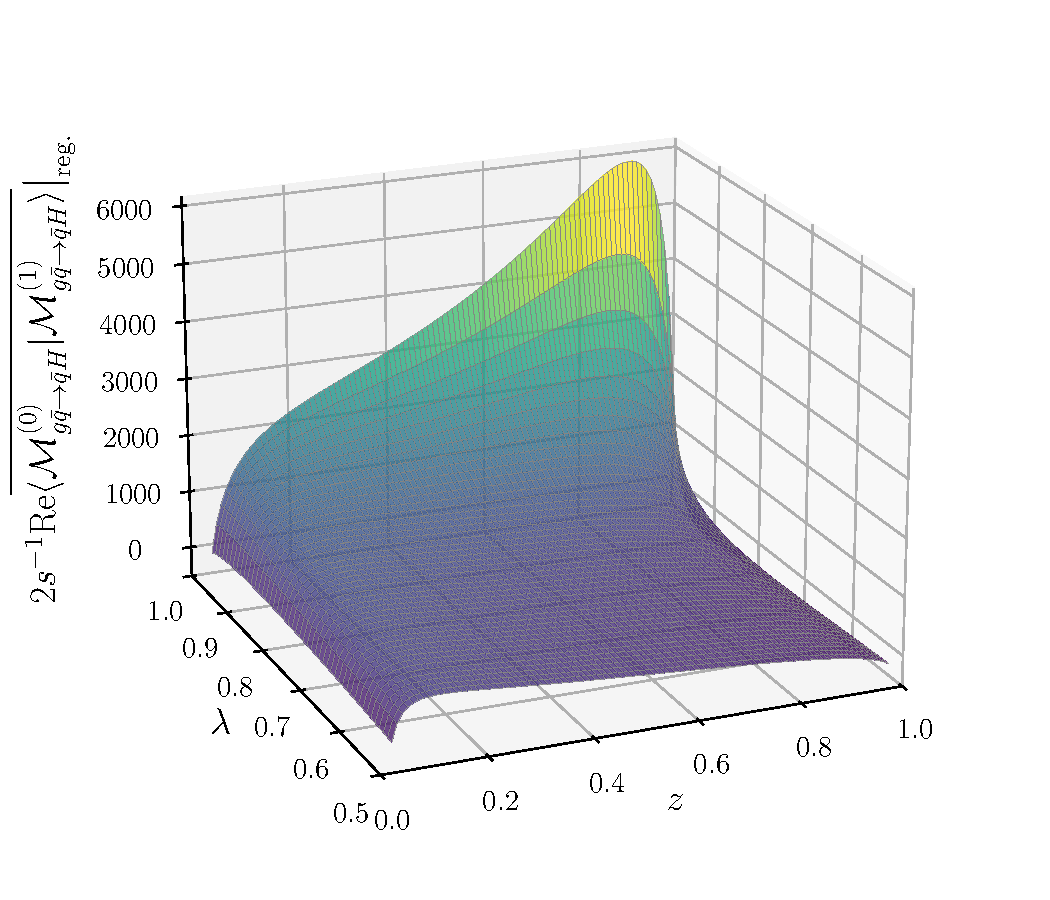
\includegraphics[width=\textwidth]{Images/RV_amplitudes/tOSbOS_gqB.pdf}
  %\captionof{figure}{}
  %\label{fig:2:luminosity}
  \end{minipage}
  \caption{Top-bottom interference contribution to the amplitudes $gg \rightarrow gH$ (top left), $\bar{q}q \rightarrow g H$ (top right), $qg \rightarrow q H$ (bottom left) and $g \bar{q} \rightarrow \bar{q}H$ (bottom right) normalized by the partonic center of mass energy $s$. Displayed is only half of the parameter space $\lambda \in [0.5, 1]$; the other half can be obtained by means of the symmetry relations in Eqs.~\eqref{eq:5:symmetry_1},\ \eqref{eq:5:symmetry_2} and\ \eqref{eq:5:symmetry_3}. For better visibility we only show grid points in the range of $\lambda \in [0.5, 0.98]$ and $z \in [0.02, 0.98]$. The amplitude is computed with on-shell renormalized quark-masses. The computational setup is described in the \hyperref[chap:notation_and_conventions]{conventions}.}
  \label{fig:5:RV_tOSbOS}
\end{figure}
%
\begin{figure}[h]
  \begin{minipage}[t]{0.49\textwidth}
  \centering
  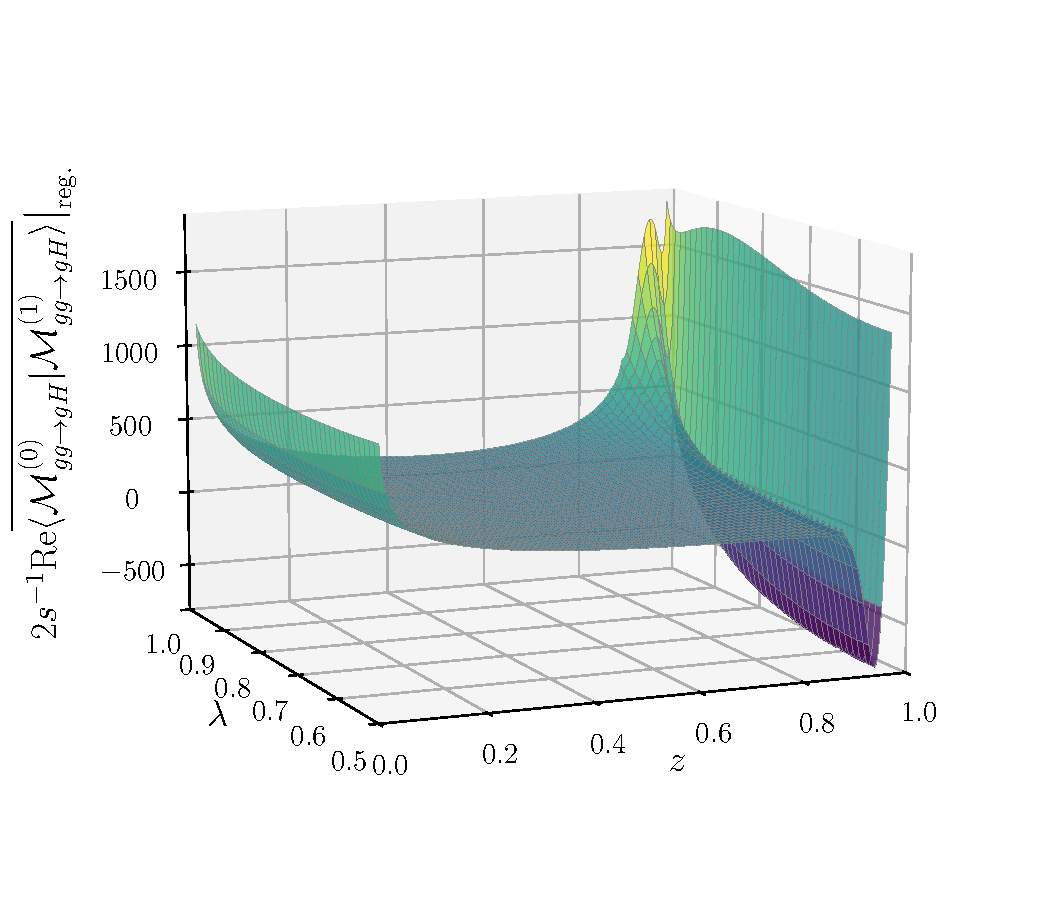
\includegraphics[width=\textwidth]{Images/RV_amplitudes/tOStOS_gg.pdf}
  %\captionof{figure}{gg}
  %\label{fig:2:PDF}
  \end{minipage}
  \begin{minipage}[t]{0.49\textwidth}
  \centering
  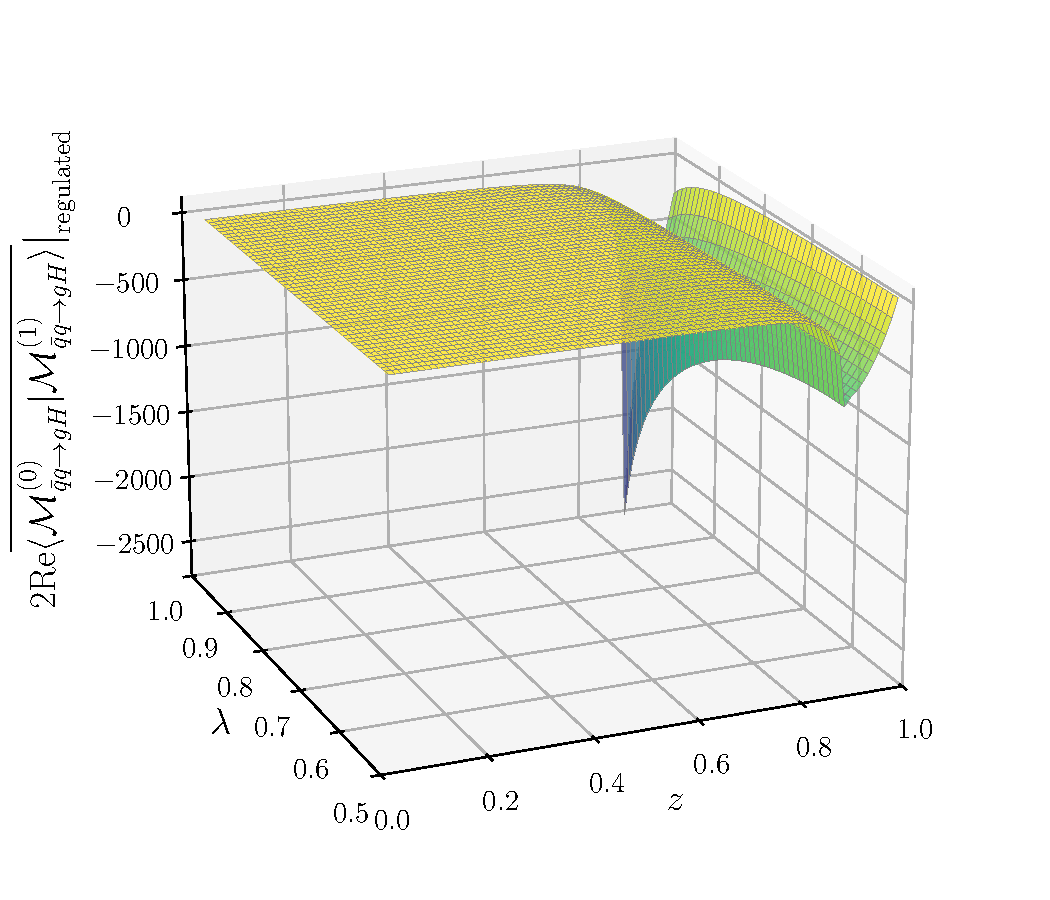
\includegraphics[width=\textwidth]{Images/RV_amplitudes/tOStOS_qBq.pdf}
  %\captionof{figure}{}
  %\label{fig:2:luminosity}
  \end{minipage}
  \begin{minipage}[t]{0.49\textwidth}
  \centering
  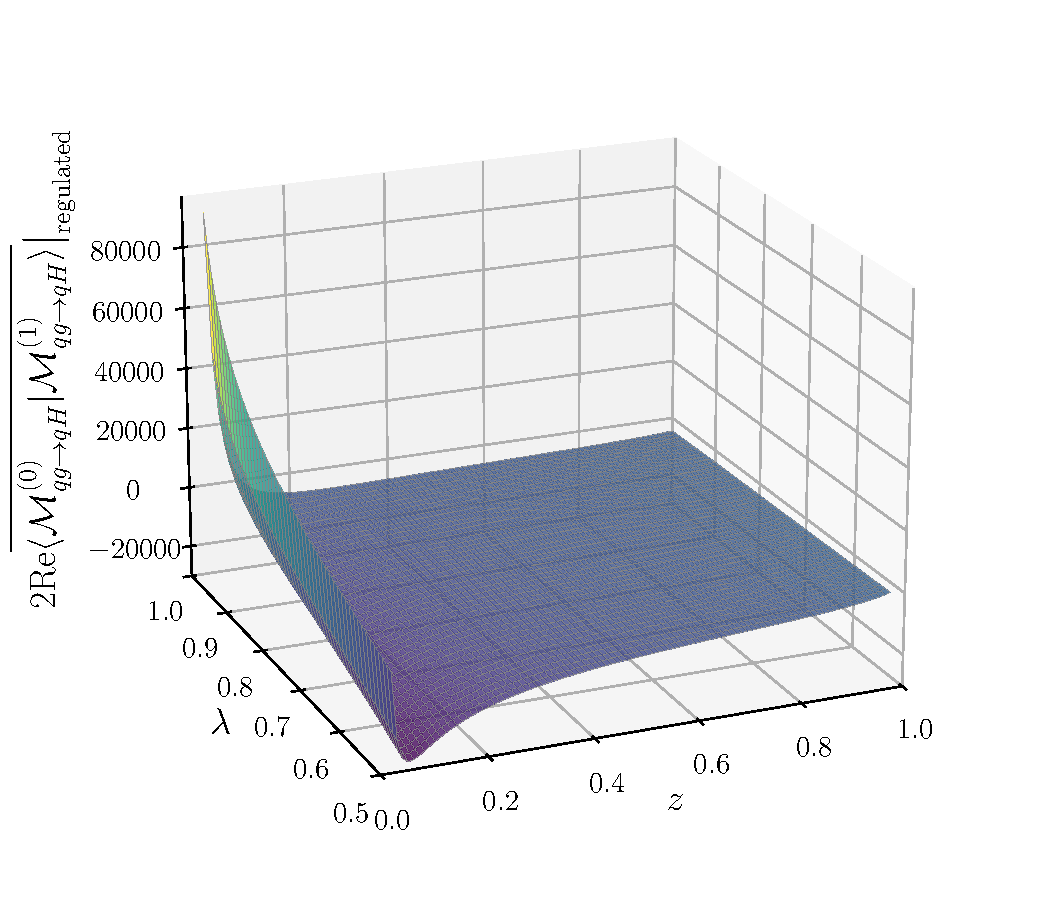
\includegraphics[width=\textwidth]{Images/RV_amplitudes/tOStOS_qg.pdf}
  %\captionof{figure}{gg}
  %\label{fig:2:PDF}
  \end{minipage}
  \begin{minipage}[t]{0.49\textwidth}
  \centering
  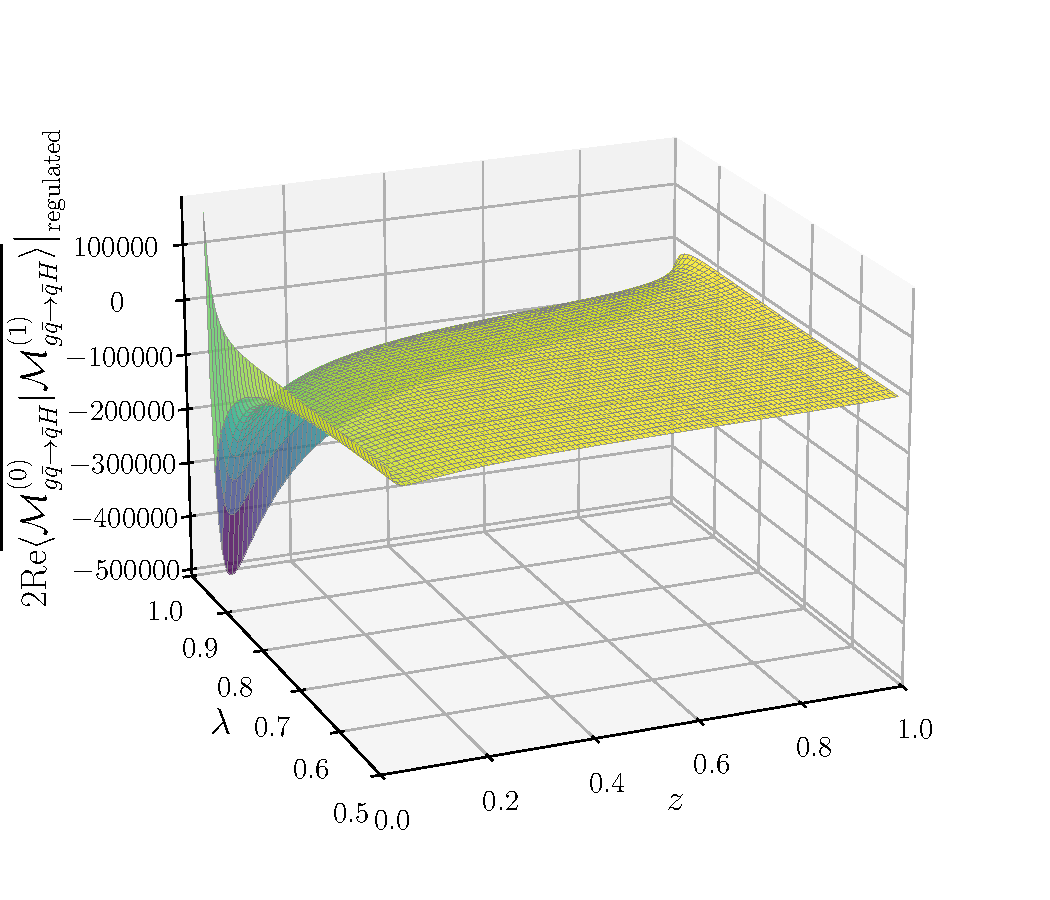
\includegraphics[width=\textwidth]{Images/RV_amplitudes/tOStOS_gqB.pdf}
  %\captionof{figure}{}
  %\label{fig:2:luminosity}
  \end{minipage}
  \caption{Same as in Fig.~\ref{fig:5:RV_tOSbOS} but for the pure-top-quark contribution to the amplitudes. Plot range for the $g g \rightarrow g H$ has been changed to $z \in [0.002, 0.965]$ and $\lambda \in [0.5, 0.98]$, for better visibility.}
  \label{fig:5:RV_tOStOS}
\end{figure}
Despite having subtracted the \acs{IR}-divergences, the amplitudes still have some residual divergences in the \acs{IR}-sensitive regions close to $z \rightarrow 0$ and $\lambda \rightarrow 1$. These divergences are however much better behaved, only showing logarithmic growth at the edges of the phase-space, and consequently can be integrated over. As expected, $\bar{q}q$-channel does not show logarithmic divergences in the soft limit $z \rightarrow 0$, since the $\bar{q} q \rightarrow H$ process was forbidden by the conservation of angular momentum (see discussion around Eq.~\eqref{eq:4:quark_form_factor}).

In the pure-top-quark contribution, the $gg \rightarrow g H$ and $\bar{q}q \rightarrow g H$ amplitudes display their most prominent features around the $t\bar{t}$-production threshold at $z_{\mathrm{threshold}} = 1 - \frac{m_H^2}{4 m_t^2} \approx = 0.87$. This aligns with our expectations, as Landau's equations predict the amplitudes to have a branch cut starting from the production threshold. The amplitudes for the $qg \rightarrow qH$ and $g \bar{q} \rightarrow \bar{q} H$ processes do not exhibit this branch cut, since here the discontinuity lies outside the physical parameter space. For the top-bottom interference contributions, the threshold region is not as feature rich, since the amplitudes with top-quark induced Higgs production are no longer squared, but instead multiplied by the bottom-quark induced Higgs production, which do not have branch cuts at the $t\bar{t}$-thresholds.

\textbf{Interpolation}\\
During the phase-space integration, we require the amplitude at any value of the parameter space not just at the grid points we computed. We can get a very accurate approximation of the amplitudes by interpolating between the grid point. To do this, we first identify a $4\times 4$ sub-grid, such that the target point lies inside the center square. We then construct cubic splines in one-dimension, say in the $\lambda$-direction using the respective grid points for fixed values of $z$. We can then use these spline fits to obtain approximations of the amplitude at the target-$\lambda$ value and the four fixed $z$-values. Afterwards, we simply use these four values to construct another cubic spline fit in the $z$-direction, which can then be used to get an approximation of the amplitude at the target phase-space point. The method is illustrated in Fig.~\ref{fig:5:interpolation} and can be straightforwardly generalized to any dimension.
\begin{figure}[h]
\centering
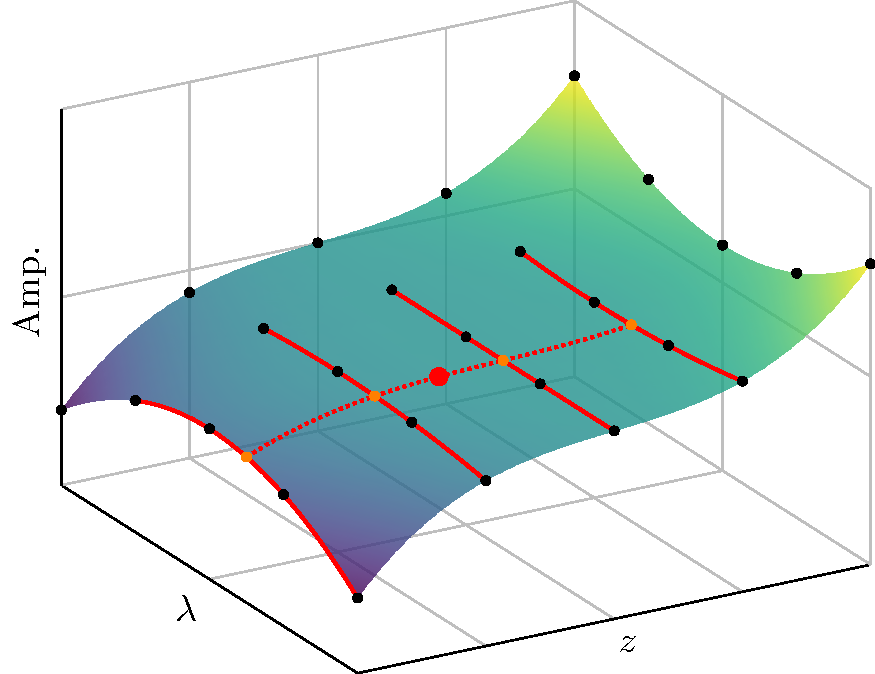
\includegraphics[scale=0.6]{Images/interpolation.pdf}
\caption{Graphical illustration of the method to perform multidimensional interpolations using cubic splines. The surface represents the actual amplitude; the black dots mark the computed grid points; the large red dot is the target phase-space point; the solid red line indicates the spline fit in the $\lambda$-direction; the orange dots mark the value of the $\lambda$-fits at the target-$\lambda$; the dashed red line marks the spline fit in the $z$-direction.}
\label{fig:5:interpolation}
\end{figure}
It should also be noted that the method does not rely on a rectangularly distributed grid samples, but just requires them to be distributed in a straight line along one direction. This is important, as our grid samples were distributed logarithmically. Furthermore, grid points which are located very close to poles of the differential equation are not being evaluated due to the contour deformation. Since the interpolation method does not require equidistant grid points we can simply ignore these points and interpolate these regions of the phase-space.

During the phase-space integration we will also encounter phase-space regions which lie outside our computed grid, making it necessary for us to extrapolate. In the infrared sensitive regions the amplitude must grow double-logarithmically, whereas in the high-energy limit $z \rightarrow 1$ it can be shown~\cite{Marzani:2008az, Harlander:2009my} that the amplitude grows as $\log^3(1 - z)$. One can therefore use a power-logarithmic \textit{Ansatz} for the extrapolation of the amplitude. We found however, that extrapolations using the cubic splines yielded results compatible within the \acs{MC} uncertainties, which is why we went with this simpler approach for our final result. The alternative extrapolation method serves as additional cross-check of the accuracy of our amplitudes in these regions of phase space.

After the interpolation, we add back the subtraction terms of Eq.~\eqref{eq:IR_regulation}, which we know fully analytically for the entire phase-space, to obtain the full amplitudes.

\subsection{The Virtual-Virtual Corrections} \label{subsec:5:virtual_virtual_corrections}
Lastly, we consider virtual-virtual corrections to the $gg \longrightarrow H$ amplitudes, that is the three-loop Higgs-gluon form factor. We can decompose the \acs{NNLO} contribution to the form factor according to the quark loops of the respective Feynman diagrams as follows:
\begin{equation}
\begin{split}
\mathcal{C}^{(2)} &=  n_t \mathcal{C}_t^{(2)} + n_t^2 \mathcal{C}_{tt}^{(2)} + n_t n_l \mathcal{C}_{tl}^{(l)} \\
& + n_b \mathcal{C}_b^{(2)} + n_b^2 \mathcal{C}_{bb}^{(2)} + n_b n_l \mathcal{C}_{bl}^{(2)} \\
& + n_t n_b \left( \mathcal{C}_{tb}^{(2)} + \mathcal{C}_{bt}^{(2)} \right).
\end{split}
\end{equation}
The first index indicates which quark flavor couples to the Higgs, and the second index---if present---marks the flavor of the the other quark loop.
That means contributions inside $\mathcal{C}_t^{(2)}$ are computed from Feynman diagrams containing only a single quark-loop with a top-quark running inside. Example Feynman diagrams for this contribution are shown in Fig.~\ref{fig:5:C_t}. $\mathcal{C}_{b}^{(2)}$ is computed by the same means only with the top-quark replaced by the bottom quark.
\begin{figure}[h]
\centering
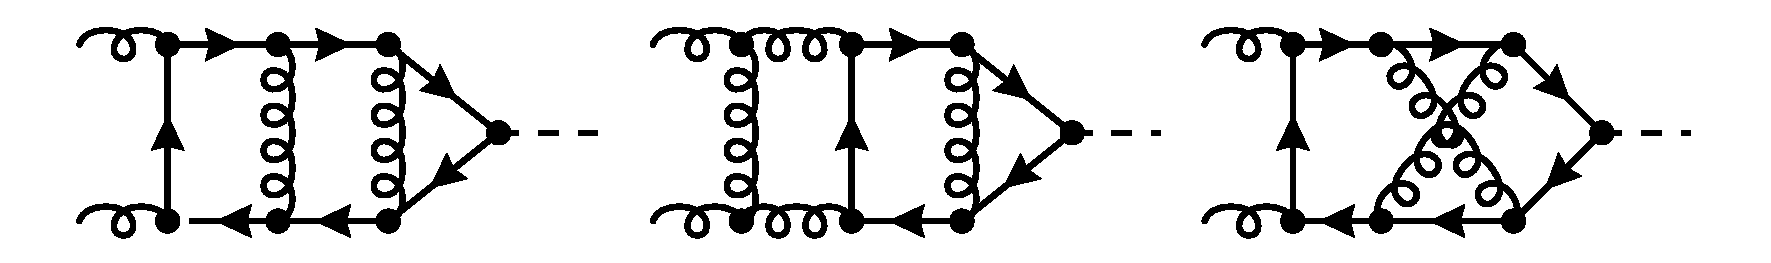
\includegraphics[width=\figurewidth]{Images/NNLO_Feynman_diagrams/C_t.pdf}
\caption{Example Feynman diagrams for contributions containing only a single heavy quark-loop.}
\label{fig:5:C_t}
\end{figure}
Similarly, $\mathcal{C}_{tt}^{(2)}$ then contains two closed top-quark loops, $\mathcal{C}_{tl}^{(2)}$ one top-quark and one light-quark loop, and so on. All Feynman diagrams containing two closed quark-loops are depicted in Fig.~\ref{fig:5:C_tt}.
%
\begin{figure}[h]
\centering
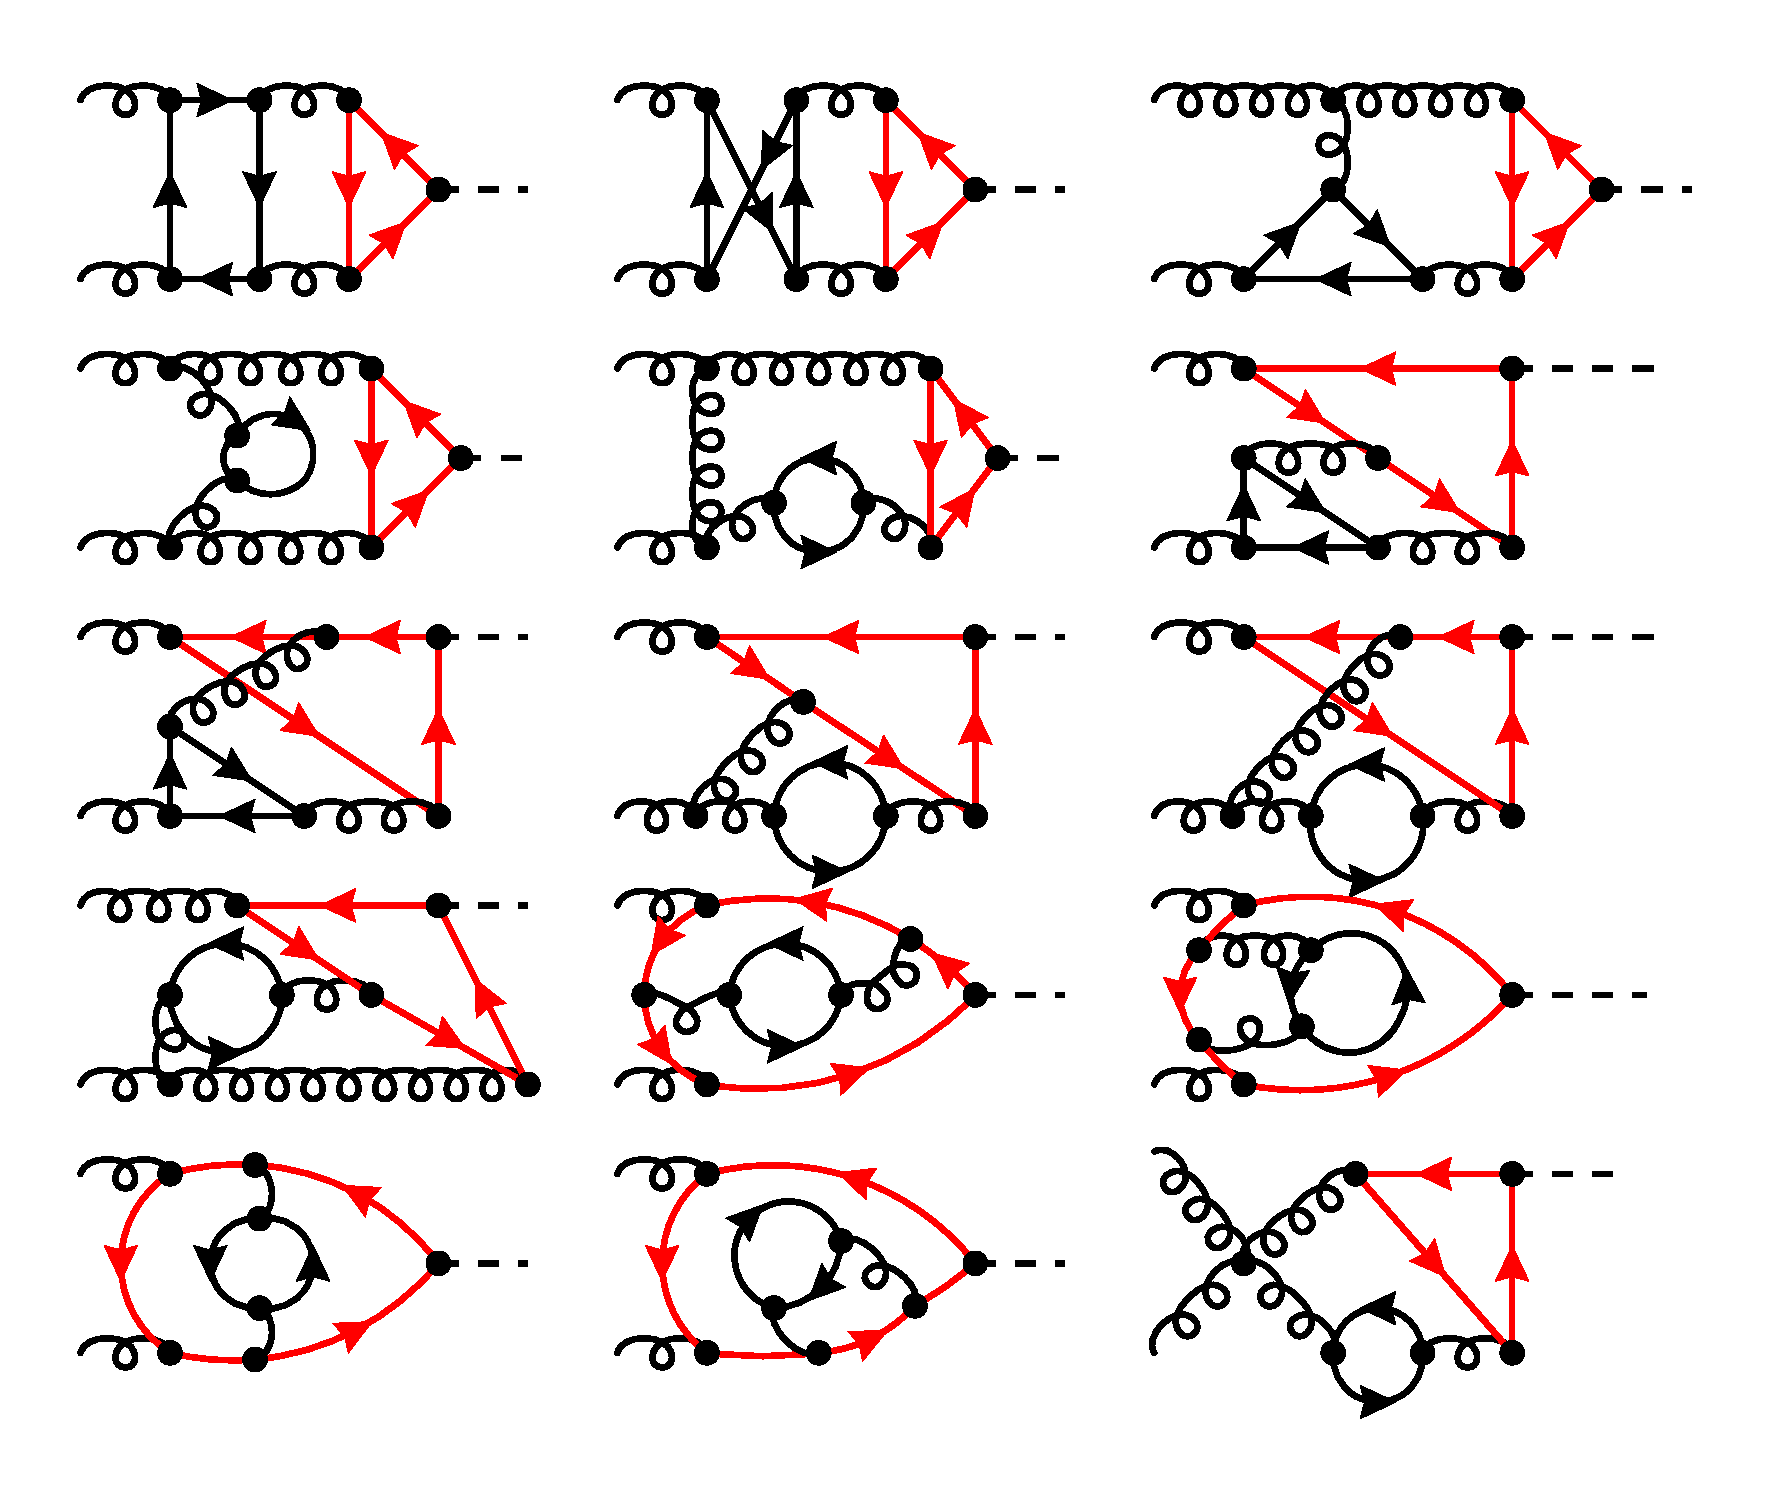
\includegraphics[width=\figurewidth]{Images/NNLO_Feynman_diagrams/C_tt.pdf}
\caption{All Feynman diagrams with two closed quark loops. The quar loop coupling to Higgs, marked in red, must be a heavy quark line, \ie\ either a top- or bottom- quark. The black quark loop can be either a top-, bottom- or light-quark. Reversed fermion flows are not explicitly drawn.}
\label{fig:5:C_tt}
\end{figure}
The $\mathcal{C}_t^{(2)}$, $\mathcal{C}_{tt}^{(2)}$, $\mathcal{C}_{tl}^{(2)}$, $\mathcal{C}_b^{(2)}$, $\mathcal{C}_{bb}^{(2)}$ and $\mathcal{C}_{bl}^{(2)}$ contributions are computed with only a single heavy quark mass, making these contributions functions of only one dimensionless variable
\begin{equation}
z_q = \frac{m_H^2}{4 m_q^2}.
\end{equation}

The $\mathcal{C}_{tb}^{(2)}$ and $\mathcal{C}_{bt}^{(2)}$ parts of the form factor on the other hand are now functions of both $z_b$ and $z_t$. They are the only instance, where we encounter non-factorizable Feynman-integrals with two-different masses in the whole cross section calculation. Note that when working in the 5\acs{FS}, the $\mathcal{C}_{tb}^{(2)}$ contribution is set to zero, because the bottom quark loop is not coupling to the Higgs.

Both, the one and two quark mass contribution have been computed recently~\cite{Czakon:2020vql,Niggetiedt:2023ywb}. They apply a method similar to what we have described in the previous chapter. They derive a set of differential equations, this time in terms $z_q$ or $z_b$ and $z_t$ and subsequently solve the differential equation numerically. The heavy-top- and the hight-energy limit are used as boundary conditions of the differential equation. The numerical samples are computed with very high precision and are then used by the authors to determine a deep asymptotic expansion in the large-mass, and the high-energy limit. For phenomenological application, both the bottom- and the top-quark mass are sufficiently far away from the threshold, that the asymptotic expansions approximate the amplitude without a relevant loss of precision. We therefore use the provided series expansions for our computations. In the public version of Ref.~\cite{Czakon:2020vql}, the amplitude is not provided with the $n_{t,b}$ tags, \ie\ it is not possible to individually extract the $\mathcal{C}_{bb}^{(2)}$ and $\mathcal{C}_{b}^{(2)}$ contribution. This is indispensable when working in the 5\acs{FS}. The obtained the amplitudes with the relevant tags through private communication with the authors of Ref.~\cite{Czakon:2020vql}.

The results for the various coefficients of the Higgs-gluon form factor are presented in Figs.~\ref{fig:5:form_factor_coefficients_t} and \ref{fig:5:form_factor_coefficients_b}. For the mixed contributions $\mathcal{C}^{(2)}_{tb}$ and $\mathcal{C}^{(2)}_{bt}$, we only display the results for a fixed \acs{OS} mass of the quark which is not coupling to the Higgs.
\begin{figure}[h]
\centering
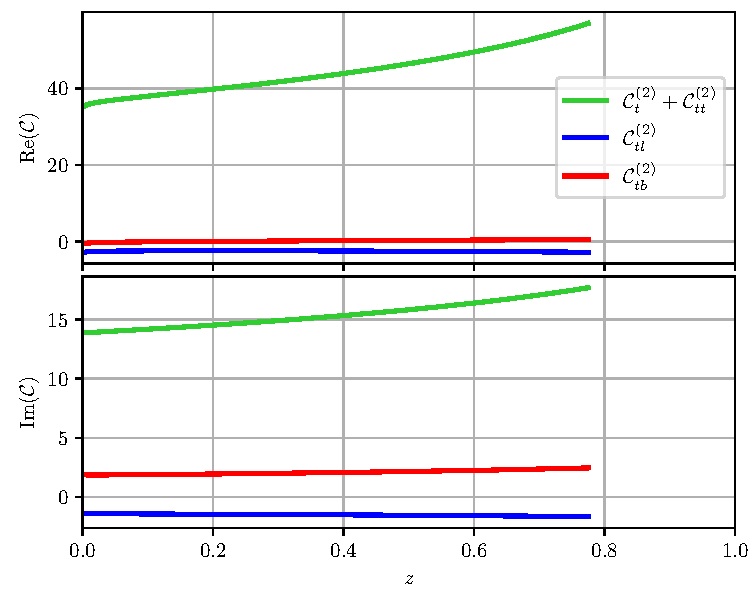
\includegraphics[width=\figurewidth]{Images/form_factor_coefficients_t.pdf}
\caption{Coefficients of the Higgs-gluon form factor in the large-mass expansion. For the $\mathcal{C}_{tb}^{(2)}$ contribution, we set the bottom quark mass to its \acs{OS}-value. Both quark masses are renormalized in the \acs{OS} scheme. \acs{IR} divergences are subtracted in the \MS\ scheme. The renormalization scale has been set to $\mu_R = m_H$. The computational setup is described in the \hyperref[chap:notation_and_conventions]{conventions}.}
\label{fig:5:form_factor_coefficients_t}
\end{figure}
\begin{figure}[h]
\centering
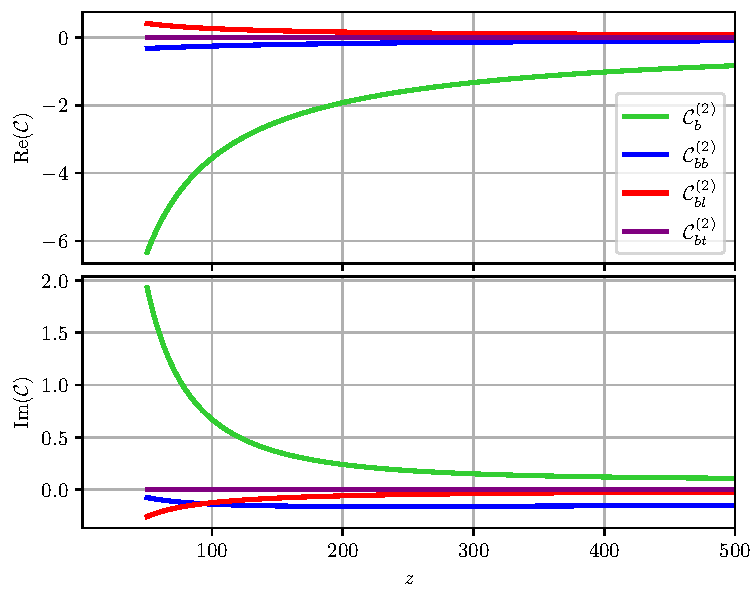
\includegraphics[width=\figurewidth]{Images/form_factor_coefficients_b.pdf}
\caption{Same as in Fig.~\ref{fig:5:form_factor_coefficients_t} but for high-energy limit. This time $\mathcal{C}_{bt}^{(2)}$ is computed using the fixed \acs{OS} top-quark mass.}
\label{fig:5:form_factor_coefficients_b}
\end{figure}
We can see that dominant contribution to the Higgs-gluon form factor comes from $\mathcal{C}_{b}$ in the high-energy limit. Since an additional fermion loop results in a power suppression of $1/N_c$, one can expect that the other coefficients $\mathcal{C}_{bb}^{(2)}, \mathcal{C}_{bl}^{(2)}$ and $\mathcal{C}_{bt}^{(2)}$ will be less significant. The observed discrepancy between the contributions is however larger than what can be expected from the color suppression, a phenomenon which is commonly observed in the computation of amplitudes. The mixed contribution $\mathcal{C}_{bt}^{(2)}$ is completely negligible, and is small even compared $\mathcal{C}_{bl}^{(2)}$ and $\mathcal{C}_{bb}^{(2)}$. This can be understood from the Appelquist-Carrazone theorem, which implies that the amplitude should be suppressed by a factor of $m_H^2/4m_t^2$.

Below the threshold, \ie\ in amplitudes where the Higgs couples to the top-quark, we also observe that the dominant coefficient is related to contributions without a second fermion loop. The imaginary part does however receive significant corrections. The mixed coefficient $\mathcal{C}_{tb}^{(2)}$ is hereby also relevant, since it is now longer suppressed by large quark masses.

Relatively recently, it was noticed by Liu and Penin that the leading logarithms, \ie\ logarithms of the form
\begin{equation}
\alphas^n \log^{n + 1} (m_b^2/m_H^2),
\end{equation}
of the high energy limit of the virtual amplitudes can be predicted and resumed to all orders of perturbation theory~\cite{Liu:2017vkm}. They identified that the cause of the leading logarithm is soft quark exchange, and they were able to rewrite the amplitude in terms of a \textit{Sudakov form factor}. The Higgs gluon form factor in the high-energy limit at leading logarithmic (\acs{LL}) accuracy reads
\begin{equation}
\mathcal{C}(z) \bigg \vert_{\text{LL}} = - Z_g^2 g(x) \left(\frac{3}{2} \frac{1}{4z} \ln^2 \left(-\frac{1}{4z} \right) \right) \mathcal{C}^{(0)}(0),
\end{equation}
where
\begin{equation}
\begin{gathered}
Z_g^2 = \exp\! \left[- \frac{C_A}{\epsilon^2} \frac{\alphas}{2 \pi} \right], \quad g(x) = {}_2F_2(1, 1;3/2,2;x/2) = 2 \sum_{n = 0}^\infty \frac{n!}{(2 n + 2)!} (2 x)^{n}, \\
\text{and} \quad x = \frac{\alphas}{4 \pi} (C_A - C_F) \ln^2\left(\frac{1}{4 z} \right).
\end{gathered}
\end{equation}
Here ${}_2F_{2}$ denotes a generalized hypergeometric function. If we expand this in $\alphas$ we obtain the same high-energy limit as in the fixed order calculations. It is interesting to compare the full fixed order results, with the leading logarithmic approximation. On the one-hand side it shows how much of the amplitude is dictated by the leading logarithm, and on the other side, if accurate, it allows us to go to very high order of perturbation theory such that we can assess the quality of the perturbation series. At $\mu_R = m_H$, with an \acs{OS} renormalized bottom quark mass and \acs{IR} divergences subtracted in the \MS\ scheme---both is irrelevant for the \acs{LL} approximation---, the form factor is\footnote{The computational setup is described in the \hyperref[chap:notation_and_conventions]{conventions}.}
\begin{equation}
\begin{split}
\mathcal{C} \left(\frac{m_H^2}{4 m_b^2}\right) &= (-0.021 + 0.030 i) \bigg \lbrace 1 + (9.237 - 0.442 i) \frac{\alphas}{\pi} + (23.571 + 40.173 i) \left(\frac{\alphas}{\pi} \right)^2 \bigg \rbrace \\
&= (-0.021 + 0.030 i) \big \lbrace 1 + (0.329 - 0.016 i) + (0.029 + 0.051 i) \big \rbrace \\[10pt]
%
\mathcal{C} \left(\frac{m_H^2}{4 m_b^2} \right) \bigg \vert_{\text{LL}} &= (-0.024 + 0.030 i) \bigg \lbrace 1 + 10.36 \frac{\alphas}{\pi} + 33.48 \left(\frac{\alphas}{\pi} \right)^2  \\
&\hspace{6cm} + 79.44 \left(\frac{\alphas}{\pi}\right)^3 + 153.93 \left( \frac{\alphas}{\pi} \right)^4 \bigg \rbrace \\
&= (-0.024 + 0.030 i) \big \lbrace 1 + 0.369 + 0.043 + 0.004 + 0.0002 \big \rbrace .
\end{split}
\label{eq:5:LL_comparison}
\end{equation}
We note that the full numbers hold in the 4\acs{FS}, for better comparability, though numerically the differences between the schemes is very small. Similarly, we omit the effects from top-quark loops, since these are also not accounted for in the \acs{LL} approximation. Again, the numerical effect is almost negligible.

Eq.~\eqref{eq:5:LL_comparison} shows that the \acs{LL} approximation is quite accurate at low perturbative order, but the quality of the approximation deteriorates at higher orders. At \acs{NNLO} only the order of magnitude of the real part is correctly predicted, whereas the imaginary part is completely off. For the top-bottom interference contribution, the imaginary part of the \acs{NNLO} corrections is however irrelevant, since the \acs{LO} amplitude below the $z=1$ threshold is real. For precision predictions, the \acs{LL} approximation is not suited, especially at high loop order.

The perturbative convergence of the amplitude seems to be relatively good. We can therefore conclude that logarithms of the form $\log^2 m_b^2/m_H^2$ do not spoil the convergence and do not necessarily need to be resumed.



\section{The 4-Flavour Scheme}\label{sec:5:4FS}
Up to this point, our discussion was mainly focused on the 5\acs{FS}, where the bottom quark is considered to be a constituent of the proton. Consequently, to avoid the appearance of large logarithms, we have set the mass of the bottom-quark to zero, except in closed bottom-quark loops that couple to the Higgs. To assess the validity of this prescription, we want to investigate the alternative 4\acs{FS}. Here the bottom-quark is consistently treated as a massive particle, and by excluding the quark from the initial state, the large \acs{IR}-logarithms will cancel in sufficiently inclusive observables. In this section, we want to summarize the necessary adaptions of our calculation for the 4\acs{FS}.

\textbf{The Real-Real Corrections} \\
In addition to the amplitudes already computed in the 5\acs{FS}, the real-real corrections now include an additional channel, in which the Higgs is produced in association with a massive $b \bar{b}$ pair. Ergo, we need amplitudes for the processes $gg \longrightarrow H b \bar{b}$, and $q \bar{q} \longrightarrow H b \bar{b}$. The second and third diagram in Fig.~\ref{fig:5:real_real} are examples of contributing Feynman diagrams. Note however, that we still require the Higgs to couple to a closed quark loop. Hence, a contribution like the one displayed in Fig.~\ref{fig:5:ggH_bbH_interference} are \textbf{not} considered in the present calculation.
\begin{figure}[h]
\centering
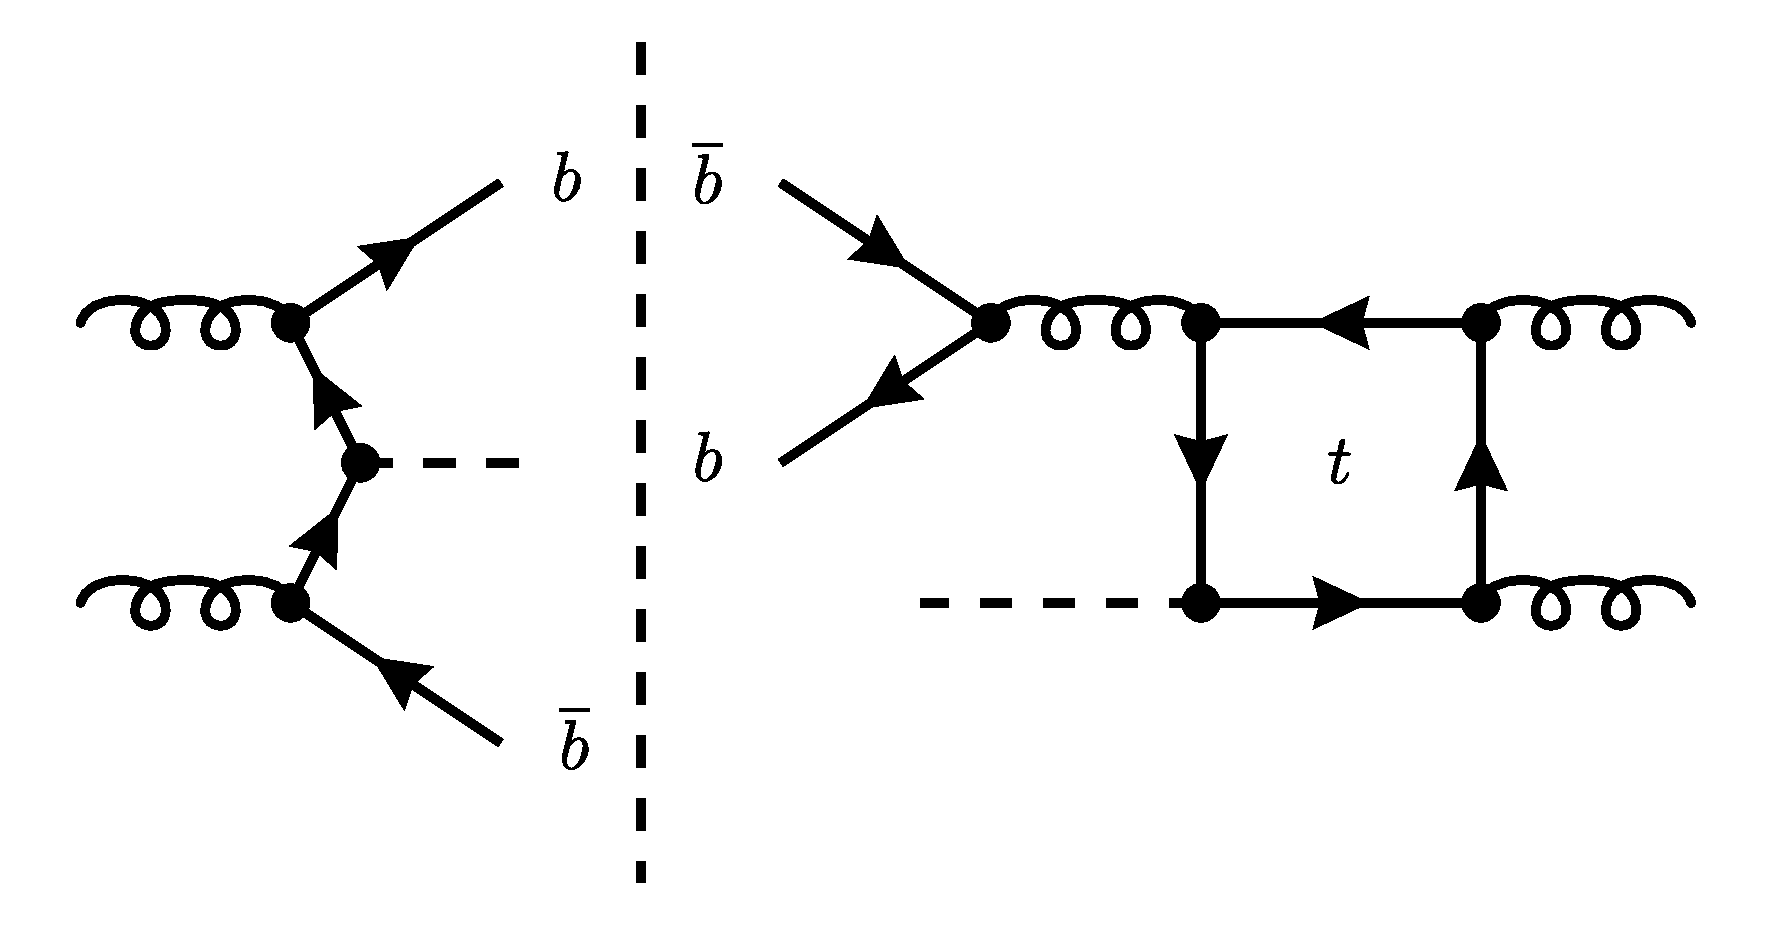
\includegraphics[scale=0.3]{Images/NNLO_Feynman_diagrams/interference_with_bbH.pdf}
\caption{Example interference diagram for a contribution to the bottom-bottom fusion channel at \acs{NLO} in the 4\acs{FS}. Because the Higgs does not couple to a closed quark loop, it is not considered a contribution to gluon-gluon fusion, but to the gluon-gluon-fusion--bottom-bottom-fusion interference.}
\label{fig:5:ggH_bbH_interference}
\end{figure}
Instead, they are considered in the interference of the bottom-bottom fusion- and gluon-gluon fusion-channel and were evaluated in the 4\acs{FS} a long time ago~\cite{Dittmaier:2003ej}.

The additional amplitudes are evaluated using the public amplitude library \texttt{RECOLA}~\cite{Actis:2016mpe}. However, the exclusion of the bottom-bottom fusion channel is not supported by \texttt{RECOLA}, and requires some out-of-the-box thinking. Our approach works by computing the amplitudes in the two-Higgs-doublet model instead of the \acs{SM}. The details of the model are irrelevant for our purposes, the only important aspect is that the model now contains a second Higgs boson $H_2$. We switch of any coupling to lighter quarks, including the bottom quark. Hence, we can compute the top-quark induced Higgs production in association of a massive $\bar{b} b$ pair. But how can we now obtain the bottom-quark induced Higgs production? The solution is to couple the second Higgs boson and rescale the momenta and masses to match the \acs{SM}, \ie\ we choose the mass of the second Higgs boson as
\begin{equation}
m_{H_2} = \frac{m_t}{m_b} m_H,
\end{equation}
and rescale all external momenta by
\begin{equation}
p_i^\mu \rightarrow \frac{m_t}{m_b} p_i^\mu.
\end{equation}
This way the mass ratio of the Higgs boson, and the internal and external quark matches the \acs{SM} ratio of $m_H$ to $m_b$. Since the mass dimension of the amplitude (without the inclusion of the \acs{VEV}) is vanishing, the global rescaling has no effect on the numerical result of the amplitude.

\textbf{The Real-Virtual Corrections} \\
Let us follow the notation from section~\ref{subsec:5:virtual_virtual_corrections} and introduce the bookkeeping parameters $n_l$, $n_b$ and $n_t$ to label light-, bottom-, and top-quark loops. The two-loop real-virtual amplitudes for the gluon-gluon fusion amplitudes then allow for the decomposition
\begin{equation}
\begin{split}
\mathcal{M}_{ij \rightarrow k H}^{(1)} &= n_t \mathcal{M}_{ij \rightarrow kH}^{(1),t} +  n_t^2 \mathcal{M}_{ij \rightarrow kH}^{(1),tt} +  n_t n_l \mathcal{M}_{ij \rightarrow kH}^{(1),tl} \\
& +  n_b \mathcal{M}_{ij \rightarrow kH}^{(1),b} +  n_b^2 \mathcal{M}_{ij \rightarrow kH}^{(1),bb} +  n_b n_l \mathcal{M}_{ij \rightarrow kH}^{(1),bl} \\
& + n_t n_b \left( \mathcal{M}_{ij \rightarrow k H}^{(1), tb} + \mathcal{M}_{ij \rightarrow k H}^{(1), bt} \right),
\end{split}
\label{eq:5:real_virtual_decomposition}
\end{equation}
where once again the first superscript indicates which quark flavor is coupling to the Higgs. In the 5\acs{FS} both $\mathcal{M}_{ij \rightarrow k H}^{(1), tb}$ and $\mathcal{M}_{ij \rightarrow k H}^{(1), tb}$ were vanishing, the $\mathcal{M}_{ij \rightarrow k H}^{(1), bt}$ was computed analytically while the rest was computed numerical. For the 4\acs{FS} we can get the $\mathcal{M}_{ij \rightarrow k H}^{(1), tb}$ contribution from the $\mathcal{M}_{ij \rightarrow k H}^{(1), bt}$ upon exchanging the top and the bottom quark, \ie\ by changing
\begin{equation}
m_t \longleftrightarrow m_b
\end{equation}
in Eqs.~\eqref{eq:5:ggg_ppp}, \eqref{eq:5:ggg_mpp}, and \eqref{eq:5:qqg_mpp}. For the remaining parts of the $2 \longrightarrow 2$ amplitudes we compute the general amplitude in Eq.~\eqref{eq:5:real_virtual_decomposition} while keeping track of the bookkeeping parameters, preserving maximal flexibly and allowing us to seamlessly change between \acs{FS}s.

\textbf{The Virtual-Virtual Corrections} \\
Similarly, the 3-loop Higgs-gluon form factor is known is a deep asymptotic series with full parametric dependence on $n_l$, $n_b$ and $n_t$. The only necessary changes to adapt the amplitude to the 4\acs{FS} is to include the $\mathcal{C}^{(2)}_{bb}$ and $\mathcal{C}^{(2)}_{tb}$ terms previously omitted.


\section{\texorpdfstring{$\MS$}{MS}-scheme}
So far, our discussion on amplitudes was limited to the on-shell renormalized quark masses. As explained in section~\ref{subsec:4:effect_of_light_quarks}, the top-bottom interference contribution is highly sensitive to the renormalization scheme, especially of the bottom quark. One of our central aims, was therefore to investigate the impact of the choice of the mass-renormalization scheme at \acs{NNLO}. In this section, we want to discuss the relevant adjustments necessary for the computation of the \MS-renormalized amplitudes.

Strictly speaking, \MS-scheme is actually a collection of renormalization schemes, as every scale $\mu$ forms a new scheme. Since $\mu$ can be varied continuously, the \acs{RG}-invarince can be leveraged in the form of the \acs{RGE}
\begin{equation}
0 = \frac{\dd \ln m_q^B}{\dd \ln \mu} \quad \Rightarrow \quad \frac{\dd \ln m_q}{\dd \ln \mu} = - \frac{\dd \ln Z_m}{\dd \alphas} \pi \bar{\beta} = 2 \alphas \frac{\dd Z_m^{(1)}}{\dd \alphas} \equiv - \gamma_m,
\end{equation}
where $\bar{\beta}$ is again the $d$-dimensional $\beta$ function of Eq.~\eqref{eq:4:d_dimensional_beta_function}, $Z_m^{(1)}$ is the residue in the $\epsilon$-expansion of the mass-renormalization constant, and $\gamma_m$ is the \textit{mass anomalous dimension}. The solution of the \acs{RGE} is given by
\begin{equation}
m_q (\mu) = m_q(\mu_0) \exp\!\left[- \int_{\mu_0}^\mu \frac{\dd \mu^\prime}{\mu^\prime} \gamma_m(\mu^\prime) \right],
\end{equation}
which truncated at one-loop yields
\begin{equation}
m_q(\mu) = m_q(\mu_0) \left( \frac{\alphas(\mu)}{\alphas (\mu_0)} \right)^{- \gamma_0/\beta_0}, \quad \text{where} \quad \gamma_0 = 6 C_F,
\end{equation}
and $\beta_0$ as in Eq.~\eqref{eq:4:beta0_and_beta1}. Beyond one-loop the differential equation becomes very challenging to solve analytically. We instead fall back to solving the differential equation numerically using the publically available software tool \texttt{CRunDec}~\cite{Schmidt:2012az}, at the highest available 4-loop accuracy.
\begin{figure}[h]
\centering
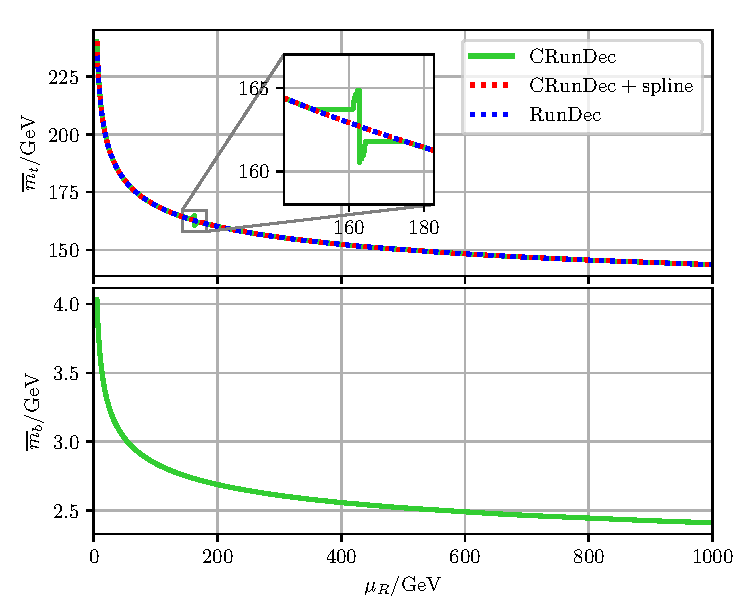
\includegraphics[width=\figurewidth]{Images/mass_running.pdf}
\caption{Running of the top- (top panel) and bottom-quark (bottom panel) mass. The solid green curve is the result computed with \texttt{CRunDec} at 4-loop accuracy. The dashed blue curve is the same but computed with \texttt{RunDec}~\cite{Chetyrkin:2000yt}. The dashed red curve uses \texttt{CRunDec} except for the region $\mu_R \in [\msMass{t}-15 \ \mathrm{GeV}, \msMass{t} + 15 \ \mathrm{GeV}]$, where we use a cubic spline instead. The computational setup is described in the \hyperref[chap:notation_and_conventions]{conventions}.}
\label{fig:5:running}
\end{figure}
Around the top-quark \MS-mass, we observed that \texttt{CRunDec} encounters numerical instabilities, which we do not observe when using its \texttt{Mathematica} sister tool \texttt{RunDec}~\cite{Chetyrkin:2000yt}. The Higgs production cross section is quite insensitive to the top-quark mass, hence we do not expect this to be of much importance. Especially considering, that in the total cross section the standard scale choice $\mu_R = m_H/2$ is below this instability region even for the scale variation. Nevertheless, we will later also introduce dynamical scales which can exceed $\msMass{t}$ for a large Higgs transverse momentum. For this reason, we bridge the problematic region around $\mu_R \in [\msMass{t} - 15 \ \mathrm{GeV}, \msMass{t} + 15\ \mathrm{GeV}]$ using a cubic spline fit which we construct from the top-quark mass at $\msMass{t} - 15 \ \mathrm{GeV}$, $\msMass{t} - 14 \ \mathrm{GeV}$,$\msMass{t} + 14 \ \mathrm{GeV}$, and $\msMass{t} + 15 \ \mathrm{GeV}$. In Fig.~\ref{fig:5:running}, we can see that the spline fit correctly reproduces the results of \texttt{RunDec} in the unstable parameter window. The evolved quark masses then enter the computed amplitudes.

Since the real-virtual amplitudes containing only a single heavy quark flavor were computed using a fixed mass ratio $m_q^2/m_H^2$ (see section~\ref{subsec:5:the_real-virtual_corrections}), we recompute the amplitude using a variety of different quark masses. In total, we computed the amplitude for nine different quark masses listed in Tab.~\ref{tab:5:masses}.
\begin{table}[h]
\centering
\begin{tabular}{cccc}
Grid mass & Value [GeV] & Approximate ratio $m_{b,t}^2/m_H^2$ & Relative error [\textperthousand] \\
\hline
$m_b$    & 4.78  & $\frac{1}{684}$ & 0.2  \\
$\overline{m}_b(m_H)$ & 2.789 & $\frac{1}{2011}$ & 0.9 \\
$\overline{m}_b(m_H/2)$ & 2.961 & $\frac{1}{1782}$ & 0.2 \\
$\overline{m}_b(m_H/4)$ & 3.170 & $\frac{1}{1557}$ & 1.0\\
$\overline{m}_b^{\text{min}}$ & 1.67 & $\frac{1}{5602}$ & 0.1 \\
$m_t$ & $172.4$ & $\frac{23}{12}$ & 4 \\
$\overline{m}_t(m_H)$ & $166.1$ & $\frac{136}{77}$ & 0.0 \\
$\overline{m}_t(m_H/2)$ & $176.2$ & $\frac{149}{75}$ & 0.0 \\
$\overline{m}_t(m_H/4)$ & $188.2$ & $\frac{213}{94}$ & 0.0
\end{tabular}
\caption{Mass ratios squared, $m_b^2/m_H^2$ and $m_t^2/m_H^2$, used for the generation of numerical values of the two-loop four-point amplitudes. We chose values corresponding to the OS masses, according to PDG recommendations \cite{Workman:2022ynf}, and \MS-masses at scales relevant for 7-point variation w.r.t.\ to a central scale of $m_H/2$. For the latter, we used $\msMass{b} = 4.18\ \text{GeV}$, as recommended by the PDG and $\msMass{t} = 162.7\ \mathrm{GeV}$. The dynamic scale \todo{Add reference ot dynamic scale} used for our differential cross-section predictions can exceed $m_H$, and reaches values of up to $1$~TeV. At this high scale, the bottom-quark mass is $\overline{m}_b(1\ \mathrm{TeV}) = 2.41~\mathrm{GeV}$. To avoid extrapolations outside our numerical grids for the amplitudes, we therefore included another mass value, $\overline{m}_b^{\text{min}}$, below this minimum.}
\label{tab:5:masses}
\end{table}
Using the interpolation method discussed in section~\ref{subsec:5:the_real-virtual_corrections}, we are now able to very quickly compute all amplitudes with high precision in a large region of the parameter space. Note that the chosen grid masses have been selected explicitly to eliminate any interpolation error for the standard fixed scale choices, \ie\ we only rely on the interpolation when using a dynamic scale. To assess the accuracy of our interpolation method, we individually removed all grid points corresponding to the masses $\overline{m}_b(m_H), \overline{m}_b (m_H/2), \overline{m}_b(m_H/4), m_t$ and reran the \acs{MC} simulation. The results differed by less than the \acs{MC} uncertainty, proofing the robustness of our interpolation method.

Evaluating on-shell renormalized amplitudes at the \MS-mass does not make them \MS-renormalized. We can however extract the \MS-renormalized amplitudes by rewriting the \acs{OS}-mass in terms of the \MS-mass
\begin{equation}
m^{\text{OS}}  = \overline{m}^{(n_m)}(\mu) \left(1 + c_1^{(n_m,n_l)} (\mu) \frac{\alphas^{(n_l)}(\mu)}{\pi} + c_2^{(n_m, n_l)}(\mu) \left( \frac{\alphas^{(n_l)}(\mu)}{\pi} \right)^2 + \mathcal{O}(\alpha^3)\right),
\label{eq:5:mOS_mMS}
\end{equation}
and then expand all amplitudes in $\alphas$ up to the required fix order. The superscripts $n_m$ and $n_l$ define which quark flavors have been decoupled from the mass and $\alphas$. The relation between the quark masses in the different renormalization schemes can be extracted using the renormalization scheme invariance of the bare quark mass, which yields the relation
\begin{equation}
Z_m^{\MS}(\mu) \overline{m}(\mu) = Z_m^{\text{OS}} m^{\text{OS}}.
\end{equation}
\Ie\ the coefficients $c_1$ and $c_2$ can simply be extracted after expanding the ratio $Z_m^{\MS}(\mu)/Z_m^{\text{OS}}$ in $\alphas$. The renormalization constants themselves have logarithmic dependencies on the \MS-\ and \acs{OS}-masses. We eliminate any residual logarithmic dependence on the \acs{OS}-mass by recursively inserting the relation~\eqref{eq:5:mOS_mMS}. Note that if the quark with the mass $m$ is not being decoupled from the running of $\alphas$, then its mass is set to zero in all contributions to the renormalization constants which feature a closed quark loop of that flavor. This is to ensure consistency with our previous prescription of quark masses.

With the renormalization constants computed in Refs.~\cite{Tarrach:1980up, Gray:1990yh} we find
\begin{equation}
\resizebox{\textwidth}{!}{
\begin{minipage}{\textwidth}
\begin{align*}
c_1^{(n_f, n_l)}(&\mu) = C_F \left(1 -\frac{3}{4} \ln\! \left(\frac{\overline{m}^{(n_f)}(\mu)^2}{\mu^2} \right) \right), \\
c_2^{(n_f, n_l)}(&\mu) = -\frac{1}{384} C_F \bigg \lbrace C_A \left(-132 \ln^2\!\left(\frac{\overline{m}^{(n_f)}(\mu)^2}{\mu^2} \right) +740 \ln\! \left(\frac{\overline{m}^{(n_f)}(\mu)^2}{\mu^2} \right) +144 \zeta (3)-1111+\pi ^2 \left( 32-96 \ln (2) \right) \right) \\
& \hspace{0.5cm} +3 C_F \bigg(-36 \ln^2\! \left(\frac{\overline{m}^{(n_f)}(\mu)^2}{\mu^2} \right) -36 \ln\! \left(\frac{\overline{m}^{(n_f)}(\mu)^2}{\mu^2} \right) -96 \zeta (3)+71+8 \pi ^2 (8 \ln (2)-5)\bigg) \\
& \hspace{0.5cm} +4 n_l T_F\left(12 \ln^2\! \left( \frac{\overline{m}^{(n_f)}(\mu)^2}{\mu^2} \right) -52 \ln\! \left( \frac{\overline{m}^{(n_f)}(\mu)^2}{\mu^2} \right) +8 \pi ^2+71\right) \bigg  \rbrace \\
& \hspace{-0.1cm}  -  \sum_{i = n_l + 1}^{n_f} \frac{1}{96} C_F T_F \bigg(12 \ln^2\! \left( \frac{\overline{m}^{(n_f)}(\mu)^2}{\mu^2} \right) -24 \ln\! \left(\frac{\overline{m}^{(n_f)}(\mu)^2}{\mu^2} \right) \ln\! \left( \frac{\overline{m}^{(n_f)}_i(\mu)^2}{\mu^2} \right) -52 \ln\! \left(\frac{\overline{m}^{(n_f)}(\mu)^2}{\mu^2} \right) \\
& \hspace{0.5cm} +32 \ln\!\left( \frac{\overline{m}^{(n_f)}_i(\mu)^2}{\mu^2} \right) +48 (x_i-1)^2 \left(x_i^2+x_i+1\right) \text{Li}_2(1-x_i)  + 48 x_i^4 \ln ^2(x_i) + 48 x_i^2 \ln (x_i)\\
& \hspace{0.5cm} -48 \left(x_i^4+x_i^3+x_i+1\right) \left(\text{Li}_2(-x_i) + \ln\!(x_i) \ln\!(x_i + 1) \right)  - 16 \pi^2 (x_i^3 + x_i) +72 x_i^2 +71\bigg),
\end{align*}
\end{minipage}
}
\refstepcounter{equation}
\tag{\theequation} \label{eq:5:c1_c2_full}
\end{equation}
where we defined $ x_i = \frac{\overline{m}^{(n_f)}_i(\mu)}{\overline{m}^{(n_f)}(\mu)}$, $n_f$ is the total number of quarks, \ie\ $n_f = 6$ in the \acs{SM} and $n_l$ is the number of light quarks, \ie\ the number of quarks which have not been decoupled in the running of $\alphas$. The sum therefore runs over all quark flavors which are decoupled from the running of $\alphas$; this includes the quark with mass $\overline{m}^{(n_f)}$ in case it is decoupled. This implies that the \acs{OS}-\MS-mass relation of the bottom-quark somehow depends on the mass of the top-quark. Since the top-quark mass is orders of magnitudes larger than the bottom-quark mass, this seems quite unphysical. The problem is that we relate the \acs{OS}-mass with the bottom-quark mass within the full $n_f = 6$ theory. Instead, we would like to relate the \acs{OS}-mass to the decoupled masses defined by
\begin{equation}
\begin{split}
\overline{m}^{(n_m)} &= \zeta_m\!\left(\alphas^{(n_m + 1)}(\mu) , \ln \frac{m^2}{\mu^2} \right) \alphas^{(n_m + 1)}(\mu), \\
\text{with} \quad \zeta_m (\alphas, L) &=  1 + \left(\frac{\alphas}{\pi}\right)^2 T_F \left[ \frac{89}{288} C_F  + \frac{5}{24} C_F L + \frac{C_F}{8} L^2 \right].
\end{split}
\end{equation}
Ones we expand our relation in $x_i \ll 1$, which we can do anyway, as all decoupling relations only hold up to power corrections, we find that all non-decoupling effects cancel as expected. The coefficients for general $n_m \le n_f$ are therefore given by Eq.~\eqref{eq:5:c1_c2_full} upon replacing $n_f \rightarrow n_m$ on the left and right-hand side.

In case we have a hierarchy among the mass scales for which $x_i \gg 1$, for example when considering the top-quark \acs{OS}-\MS-mass relation in the 4\acs{FS}, we can expand the expression yielding
\begin{equation}
\resizebox{\textwidth}{!}{
\begin{minipage}{\textwidth}
\begin{align*}
c_1^{(n_m, n_l)}(&\mu) = C_F \left(1 -\frac{3}{4} \ln\! \left(\frac{\overline{m}^{(n_m)}(\mu)^2}{\mu^2} \right) \right), \\
c_2^{(n_m, n_l)}(&\mu) = -\frac{1}{384} C_F \bigg \lbrace C_A \left(-132 \ln^2\!\left(\frac{\overline{m}^{(n_m)}(\mu)^2}{\mu^2} \right) +740 \ln\! \left(\frac{\overline{m}^{(n_m)}(\mu)^2}{\mu^2} \right) +144 \zeta (3)-1111+\pi ^2 \left( 32-96 \ln (2) \right) \right) \\
& \hspace{2.5cm} +3 C_F \bigg(-36 \ln^2\! \left(\frac{\overline{m}^{(n_m)}(\mu)^2}{\mu^2} \right) -36 \ln\! \left(\frac{\overline{m}^{(n_m)}(\mu)^2}{\mu^2} \right) -96 \zeta (3)+71+8 \pi ^2 (8 \ln (2)-5)\bigg) \\
& \hspace{2.5cm} +4 n_l T_F\left(12 \ln^2\! \left( \frac{\overline{m}^{(n_m)}(\mu)^2}{\mu^2} \right) -52 \ln\! \left( \frac{\overline{m}^{(n_m)}(\mu)^2}{\mu^2} \right) +8 \pi ^2+71\right) \bigg \rbrace \\
& \hspace{-1cm}   - \frac{1}{96} C_F T_F \bigg \lbrace 72  \\
& \hspace{-0.5cm} +  \sum_{i = n_l + 1}^{n_m}  \left[71 - 20 \ln\! \left( \frac{\overline{m}^{(n_m)}(\mu)^2}{\mu^2} \right) - 12 \ln^2\! \left( \frac{\overline{m}^{(n_m)}(\mu)^2}{\mu^2} \right) + 8 \pi^2 (1 - 3 x_i) + 16 \ln (x_i) \left(4 - 3 \ln\! \left( \frac{\overline{m}^{(n_m)}(\mu)^2}{\mu^2} \right) \right) \right] \bigg \rbrace.
\end{align*}
\end{minipage}
}
\refstepcounter{equation}
\tag{\theequation} \label{eq:5:c1_c2_expanded}
\end{equation}
The sum once again runs over all quark flavors decoupled from the running of $\alphas$, with masses less or equal than $m$. We once again underscore that these are not the standard relations between the pole and the \MS-masses, thanks to our prescription of the bottom quark mass in loops that do not couple to the Higgs. However, the standard relations follow upon replacing
\begin{equation}
n_l \longrightarrow n_l - 1
\end{equation}
in Eqs.~\eqref{eq:5:c1_c2_full} and \eqref{eq:5:c1_c2_expanded}.

For convenience of the reader we also provide the numerical values for the top- and bottom-quark mass scheme relations in the 4 and 5\acs{FS}s
\begin{align}
\mathrm{5FS: }\ m_t &= \overline{m}^{(6)}_t(\overline{m}^{(6)}_t) \left(1 +  1.333 \times \frac{\alphas^{(5)}}{\pi} + 8.237 \times \left(\frac{\alphas^{(5)}}{\pi}\right)^2 + \BigO{\alphas^3} \right) \notag \\
&= \left(162.7 + 7.493 + 1.608 \right) \ \mathrm{GeV},  \label{eq:5:mtOS_mtMS_5FS} \\[10pt]
\mathrm{4FS: }\ m_t &= \overline{m}^{(6)}_t(\overline{m}^{(6)}_t) \left(1 +  1.333 \times \frac{\alphas^{(4)}}{\pi} + 8.864 \times \left(\frac{\alphas^{(4)}}{\pi}\right)^2 + \BigO{\alphas^3} \right) \notag \\
&= \left(162.7 + 7.434 + 1.694 \right) \ \mathrm{GeV},  \label{eq:5:mtOS_mtMS_4FS} \\[10pt]
\mathrm{5FS: }\ m_b &= \overline{m}^{(5)}_b(\overline{m}^{(5)}_b) \left(1 +  1.333 \times \frac{\alphas^{(5)}}{\pi} + 8.132 \times \left(\frac{\alphas^{(5)}}{\pi}\right)^2 + \BigO{\alphas^3} \right) \notag \\
&= \left(4.18 + 0.398 + 0.174 \right) \ \mathrm{GeV},  \label{eq:5:mbOS_mbMS_5FS} \\[10pt]
\mathrm{4FS: }\ m_b &= \overline{m}^{(5)}_b(\overline{m}^{(5)}_b) \left(1 +  1.333 \times \frac{\alphas^{(4)}}{\pi} + 9.278 \times \left(\frac{\alphas^{(4)}}{\pi}\right)^2 + \BigO{\alphas^3} \right) \notag \\
&= \left(4.18 + 0.443 + 0.245 \right) \ \mathrm{GeV}. \label{eq:5:mbOS_mbMS_4FS} \\[10pt] \notag
\end{align}
We stress that the top-quark masses on the right-hand side of Eqs.~\eqref{eq:5:mtOS_mtMS_5FS} and \eqref{eq:5:mtOS_mtMS_4FS} are not decoupled, and for the bottom-quark masses in Eqs.~\eqref{eq:5:mbOS_mbMS_5FS} and\ \eqref{eq:5:mbOS_mbMS_4FS}, only the top-quark is decoupled. The first two expansion parameters already indicate a relatively good perturbative convergence for the top-quark, whereas the bottom quark receives quite large correction, a phenomenon which actually worsens with higher orders of perturbation theory~\cite{Marquard:2015qpa,Marquard:2016vmy}. The top quark mass is not relevantly effected by the choice of the \acs{FS}, whereas we see a slight shift of the bottom-quark mass of around $2\%$.

We can now insert the \acs{OS}-\MS-mass relation into the \acs{OS}-renormalized amplitudes and subsequently expand in $\alphas$, yielding the relation between the amplitudes in the two schemes
\begin{equation}
\begin{split}
  & \mathcal{M}^{\overline{\text{MS}}}(\overline{m}(\mu)) = \mathcal{M}^{\text{OS}}(\overline{m}(\mu)) + \delta \mathcal{M} (\overline{m}(\mu)), \\
  & \delta \mathcal{M}^{(1)} (\overline{m}(\mu)) = \overline{m}(\mu)c_1(\mu) \frac{\alpha_s(\mu)}{\pi}\frac{\mathrm{d} \mathcal{M}^{\text{OS},(0)}}{\mathrm{d} m} \bigg \vert_{m = \overline{m}(\mu)} , \\
  & \delta \mathcal{M}^{(2)} (\overline{m}(\mu)) = \overline{m}(\mu) \left[ c_1(\mu) \frac{\alpha_s(\mu)}{\pi} \frac{\mathrm{d} \mathcal{M}^{\text{OS},(1)}}{\mathrm{d} m}\bigg \vert_{m = \overline{m}(\mu)}  + c_2(\mu) \left(\frac{\alpha_s(\mu)}{\pi}\right)^2 \frac{\mathrm{d}\mathcal{M}^{\text{OS},(0)}}{\mathrm{d}m}\bigg \vert_{m = \overline{m}(\mu)}  \right] \\
  & \hspace{7.5cm}+ \frac{1}{2}\left(\overline{m}(\mu) c_1(\mu) \frac{\alpha_s(\mu)}{\pi} \right)^2 \frac{\mathrm{d}^2 \mathcal{M}^{\text{OS},(0)}}{\mathrm{d} m^2} \bigg \vert_{m = \overline{m}(\mu)} .
\end{split}
\label{eq:5:MMS_to_MOS}
\end{equation}
The relevant \acs{LO} and \acs{NLO} amplitudes are known fully analytically. For the Higgs-gluon form factor, we use a deep asymptotic expansion in the high-energy or large-mass limit,  and then perform the necessary mass derivatives fully automized using \texttt{Mathematica}. For the one-loop real-corrections, we apply the derivatives already applied at the level of Feynman rules using \texttt{DiaGen/IdSolver}. Taking mass derivatives, is necessary for the large-mass expansion, so the feature is already implemented. The resulting derivatives are then processed using the same tool chain described in section~\ref{subsec:5:the_real-virtual_corrections}. In a nutshell, we project to form factors, use \acs{IBP}s to reduce the integrals to master integrals, and insert the solutions to the appearing one-loop integrals.


\section{Performing the Phase-Space Integration}
Once, we collected all the relevant amplitudes, we perform the phase-space integration to obtain cross sections. We perform the phase-space integration numerically using \acs{MC} methods. The \acs{IR}-singularities arising during the integration are handled using the \textit{sector-improved residue subtraction scheme}\footnote{See section~\ref{subsec:2:phase_space_integration} for a brief review on subraction schemes.}~\cite{Czakon:2010td}, implemented in the private software package \texttt{Stripper}.

Typically, \texttt{Stripper} runs the \acs{MC} simulation at a fixed renormalization scale, and then evolves the final result to other desired scales automatically based on the provided lower order amplitudes. This procedure is however only implemented if the involved masses are renormalization scale independent, hence it is not fully automatized in the \MS-scheme. Each renormalization scale is therefore run individually.

For the top-quark induced Higgs-production cross section we subtract the \acs{rHTL} limit already on the integrand level. Since the \acs{rHTL} already captures the bulk of the cross section, this massively improves the \acs{MC} uncertainties. To get the total cross section we can then add back the \acs{rHTL} cross section after performing the phase-space integration. The \acs{rHTL} cross sections on the other hand can be evaluated extremely efficiently by public software tools like \texttt{SusHi} or \texttt{iHixs}.

